\chapter{Estudo 4: desenvolvimento, versões históricas e análises complementares}\label{ap:gzcmd}

\section{Política histórica v3}\label{sec:e4-ap-historico}

Esta seção reúne o que sustenta a comparação histórica da v3, política dos experimentos de desenvolvimento, e não integra a avaliação de ASR. As etapas da v3 estão no Algoritmo~\ref{alg:gzcmd-pipeline}, e as fórmulas, no Apêndice~\ref{sec:apendice-formalizacao}.

No desenho da v3, a estimativa $p_{cal}$ da sigmoide ajustada nas âncoras (Seção~\ref{sec:e4-calibracao}) delimitava três regiões decisórias por dois limiares: $t_{high}$ (limiar superior de confiança) e $t_{low}$ (limiar inferior de confiança); na execução histórica, $p_{cal}$ foi a transformação da nota final por \textit{Platt scaling} supervisionado, e não a sigmoide das âncoras (Algoritmo~\ref{alg:gzcmd-pipeline}). Pares com $p_{cal}\geq t_{high}$ eram classificados como de alta confiança de par verdadeiro; pares com $p_{cal}\leq t_{low}$, como não pares; e os intermediários ($t_{low}<p_{cal}<t_{high}$) eram avaliados pelo \textit{expected loss engine}. Essas regiões de probabilidade não redefinem a faixa intermediária da nota final do Comparador de Registros (CdR), $[5,9)$, nem se confundem com as seis faixas operacionais dessa nota, usadas para calibração, perfil de erro do revisor e monitoramento.

Os limiares convencionais de nota 5 e 9 não constituíam duas guardas rígidas na v3: o limiar da guarda de aceitação era 10,0, com exigências adicionais de consistência, e apenas quatro pares foram aceitos por essa guarda; a guarda inferior de nota era $<3$, não $<5$. O lote selecionado pelo motor incluiu 22 pares com nota final do CdR $\geq9$, sendo um com nota $\geq10$ e 21 em $[9,10)$. Na faixa intermediária da nota final, definida por $5\leq\text{nota}<9$, 2.821 pares foram rejeitados pela guarda temporal no artefato histórico. Esse descarte decorre da guarda temporal, que atua pela data e não pelo valor esperado da revisão (EVR, definido adiante), e não se atribui a $EVR\leq0$. Esses resultados distinguem as decisões históricas dos critérios pretendidos; a v3.1 corrige os cortes de nota e separa as guardas das decisões automáticas por custo esperado.

\subsection{Regras de guarda determinísticas da versão v3}
\label{sec:e4-regras-guarda}

Na versão v3, as regras de guarda incorporavam conhecimento epidemiológico e restrições de consistência que se sobrepunham ao classificador em casos críticos, com limiares configuráveis em YAML. Elas não descrevem as guardas de nota e probabilidade da v3.1 (Seção~\ref{sec:e4-politica-v31}).

\begin{itemize}
\item \textbf{Filtro de homonímia}: na v3, nota final pelo menos 7, subescores disponíveis de nascimento todos nulos, diferença conhecida entre anos de nascimento maior que 5 e subescores disponíveis de endereço todos nulos determinavam encaminhamento obrigatório à revisão, não exclusão. A regra combina nota, discordância de nascimento e ausência de evidência de endereço, não exige divergência de nome ou nome da mãe e não se aplica quando uma guarda anterior já decidiu o par; a implementação usa os indicadores \texttt{dtnasc\_all\_zero} e \texttt{endereco\_zero} quando presentes e, na sua ausência, trata valores faltantes como zero, exigindo ao menos uma coluna em cada grupo (\path{gzcmd/guardrails.py});
\item \textbf{Filtro temporal}: pares com data de óbito precedendo a data de diagnóstico em mais de 180 dias eram forçados para a decisão \texttt{NONMATCH}; no recorte municipal (Sinan-TB de 2013 a 2022, SIM de 2019 a 2022), essa regra não removeu PAR~=~1 ou 2. Como a manutenção de pares com notificação posterior ao óbito no processo de origem não está documentada (Seção~\ref{sec:fontes-dados}), a ausência de remoção não avalia a segurança da regra, e notificações do Sinan-TB registradas após o óbito poderiam ser indevidamente excluídas, possibilidade não examinada nos dados deste estudo.
\end{itemize}

A cardinalidade N:1 e o encaminhamento de candidatos concorrentes por margem de probabilidade foram previstos, mas não implementados. O parâmetro \texttt{conflict\_margin\_delta}, de 0,03 no YAML histórico, não é consumido pelo motor; não se executou a regra de $\Delta p<0{,}05$ descrita no desenho. Dos 21 falsos positivos (FP) de ASR na vigilância, um compartilha REFREC com um PAR~=~1 aceito acima do corte e nenhum compartilha COMPREC; os outros 20 não compartilham nenhum desses identificadores com essa referência. Nenhum dos quatro FP da confirmação compartilha esses identificadores com os PAR~=~1 aceitos. Essa contagem não avalia conflitos entre novas aceitações nem demonstra que uma restrição N:1 eliminaria os FP (\path{data/fp_cardinalidade.json}).

\subsection{\textit{Expected loss engine} da versão v3}
\label{sec:e4-motor-politica}

Na versão v3, o motor decisório substituía limiares fixos pela minimização da \textit{expected loss}, o custo médio de cada ação possível dada a incerteza sobre o verdadeiro status do par. Três ações eram consideradas: aceitar como vínculo ($a_M$), rejeitar ($a_N$) ou encaminhar para revisão ($a_R$). Os parâmetros de custo, estritamente positivos, eram $C_{FP}$ (falso positivo), $C_{FN}$ (falso negativo) e $C_{LLM}$ (revisão de um par pelo modelo de linguagem de grande porte, LLM). As proporções condicionais de erro do módulo de revisão eram $e_{FP}\in[0,1]$ (probabilidade de aceitar um não par) e $e_{FN}\in[0,1]$ (probabilidade de rejeitar um par verdadeiro). Para $p\in[0,1]$, as perdas de cada ação eram estimadas por:
\[
\mathcal{L}(a_M\mid p)=(1-p)\,C_{FP},
\quad
\mathcal{L}(a_N\mid p)=p\,C_{FN},
\]
\[
\mathcal{L}(a_R\mid p)=C_{LLM}+(1-p)e_{FP}C_{FP}+pe_{FN}C_{FN}.
\]

A Tabela~\ref{tab:cap8-custos} resume os valores históricos dos parâmetros de custo nos dois modos operacionais, que representavam a assimetria de consequências. No modo de vigilância, atribuía-se à perda de um par verdadeiro ($C_{FN}=50$) custo cinco vezes maior que ao falso positivo ($C_{FP}=10$), que pode encerrar como óbito a notificação de outra pessoa e fazer parecer notificado um óbito sem notificação. No modo de confirmação, o custo de um falso positivo ($C_{FP}=100$) superava o do falso negativo ($C_{FN}=20$). Esses valores expressavam preferências de decisão, não custos econômicos medidos.

\begin{table}[!ht]
\centering
\caption{Parâmetros históricos da versão v3 do GZ-CMD (política de três ações: aceitar como vínculo, rejeitar (\texttt{NONMATCH}) e revisão por modelo de linguagem). Os intervalos de erro indicados abrangem as faixas de nota inferior a 9; a política v3.1 (quatro ações, com revisão humana distinta da revisão por modelo de linguagem) é descrita na Seção~\ref{sec:e4-politica-v31}. Fonte: \texttt{gzcmd/gzcmd\_v3\_config.yaml}, no \textit{commit} histórico \texttt{e7700120}; $C_{LLM}=0{,}25$ é o valor da v3 histórica, e os custos das análises atuais usam $C_{LLM}=0{,}005$.}
\label{tab:cap8-custos}
\begin{tabular}{|l|c|c|c|c|c|}
\hline
Modo & $C_{FP}$ & $C_{FN}$ & $C_{LLM}$ & $e_{FP}$ (faixa) & $e_{FN}$ (faixa) \\
\hline
Vigilância & 10 & 50 & 0,25 & 0,02 a 0,10 & 0,06 a 0,15 \\
\hline
Confirmação & 100 & 20 & 0,25 & 0,02 a 0,10 & 0,06 a 0,15 \\
\hline
\end{tabular}
\end{table}

As proporções de erro residual do revisor ($e_{FP}$, $e_{FN}$) eram hipóteses de configuração fixadas por faixa da nota final do CdR, e não estimativas do revisor usado nos experimentos; a indexação seguia essa nota, sem usar o escore do OpenRecLink nem diretamente $p_{cal}$. Com proporções constantes dentro de cada faixa, $\mathcal{L}(a_R\mid p)$ é afim por partes (Proposição~\ref{prop:review-loss-affine}). A regra de menor perda estimada na versão v3 era
\[
\delta^*(p)=\arg\min_{a\in\{a_M,a_N,a_R\}}\mathcal{L}(a\mid p).
\]
Definia-se ainda o valor esperado da revisão,
\[
EVR(p)=\min\{\mathcal{L}(a_M\mid p),\mathcal{L}(a_N\mid p)\}-\mathcal{L}(a_R\mid p),
\]
e $EVR(p)>0$ indicava candidato à revisão, sujeito ao orçamento disponível.

Na execução, pares com decisão de base \texttt{MATCH} e $p$ abaixo de 0,85 (0,95 na confirmação), ou \texttt{NONMATCH} e $p$ acima de 0,15 (0,10), e os de risco de homonímia também eram encaminhados. A seleção priorizava a homonímia, depois esses limites e, por último, $EVR>0$, com ordenação por EVR dentro de cada prioridade (\path{gzcmd/gzcmd_v3_policy_engine.py}, com a configuração em \texttt{gzcmd/gzcmd\_v3\_config.yaml}). Nos empates de perda, preferia-se a melhor ação automática; entre aceitar e rejeitar, aceitava-se. A concavidade de $EVR$ vale dentro de cada faixa, sem garantia global (Proposição~\ref{prop:evr-concavity}). Essa formulação histórica não inclui a revisão humana como quarta ação, introduzida na v3.1.

A alocação do orçamento na política v3.1 é aplicada por janela, com controle do consumo entre lotes, e os limites de LLM valem para pares, não para chamadas individuais de API. Ela prioriza os LLM que vencem a comparação nominal, pelo ganho sobre a melhor alternativa que não seja LLM; entre os demais pares, priorizam-se os ganhos da revisão humana sobre a melhor ação ainda disponível. Se a capacidade humana se esgota, usa-se LLM quando há capacidade e ganho sobre a decisão automática; caso contrário, aplica-se a melhor ação automática. Trata-se de prioridade gulosa determinística, não de otimização global conjunta. O limite humano cobre apenas encaminhamentos diretos, sem reservar vagas para futuros inconclusivos do LLM, cuja carga é contabilizada separadamente.

\subsection{Fluxo operacional da versão v3}
\label{sec:e4-fluxo}

O fluxo histórico da versão v3 do GZ-CMD (representação, classificação, calibração, atribuição de faixa, regras de guarda, triagem por \textit{expected loss}, revisão assistida e decisão final) está formalizado como desenho avaliado no Algoritmo~\ref{alg:gzcmd-pipeline}, e a política v3.1 consta do Algoritmo~\ref{alg:gzcmd-v31}. A classificação fora da amostra (OOF) e as quatro ações da v3.1 substituem os ajustes e a triagem históricos (Seções~\ref{sec:e4-classificador-oof} e~\ref{sec:e4-politica-v31}).

\section{Calibração sem gabarito: âncoras e Beta por momentos}\label{sec:e4-ap-ancoras}

Esta seção reúne a calibração por conjuntos âncora, avaliada como alternativa à isotônica supervisionada que a política v3.1 adota, e sua extensão Beta. Os valores da nota final constam de \texttt{data/ancoras\_beta\_validacao.csv}.

\subsection{Calibração por âncoras}
\label{sec:e4-calibracao}

Em contraste com o esquema clássico de Fellegi e Sunter \cite{Fellegi1969theory}, a proposta inicial adotou calibração discriminativa dos escores brutos por uma sigmoide,
\[
p_{cal}(s)=\frac{1}{1+\exp\left(-\left(\alpha s+\beta\right)\right)},
\]
estimativa de $P(y{=}1\mid s)$, a probabilidade de que o potencial par seja um par verdadeiro dado o escore observado. A forma sigmoide é uma hipótese de modelagem. Seus parâmetros são ajustados em conjuntos âncora, subconjuntos de pares com status presumido de alta confiança por escore extremo: os positivos ($A^+$, escore elevado) e os negativos ($A^-$, escore muito baixo). O ajuste dispensa novos \textit{labels} em tempo de operação e preserva a ordenação dos escores, mas sua interpretação probabilística exige validação com \textit{labels}, tendo a isotônica supervisionada como referência; a dispensa de novos \textit{labels} na operação não demonstra calibração absoluta sem supervisão. O ajuste sigmoide por momentos nas âncoras é distinto do \textit{Platt scaling} supervisionado da nota e de ASR-Platt, que calibra o logit da probabilidade bruta abaixo do corte e é tratado como sensibilidade (Seção~\ref{sec:e4-arranjo-metodo}).

Os parâmetros $\alpha$ e $\beta$ são obtidos por restrições de média alvo sobre as âncoras,
\[
\mathbb{E}_{s\in A^+}[\sigma(\alpha s+\beta)] = r^+,
\qquad
\mathbb{E}_{s\in A^-}[\sigma(\alpha s+\beta)] = r^-.
\]
Os alvos satisfazem $0<r^-<r^+<1$, pois os valores 0 e 1 não são atingidos por uma sigmoide com parâmetros finitos. Essas restrições controlam apenas as duas médias nas âncoras, sem garantir calibração local na região intermediária nem estabilidade sob deriva; as limitações de identificabilidade, de estabilidade numérica e de contaminação estão no Apêndice~\ref{sec:apendice-formalizacao} (Proposição~\ref{prop:anchor-contamination-bias}).

\subsection{Validação empírica dos conjuntos âncora}
\label{sec:e4-validacao-ancoras}

A Tabela~\ref{tab:cap8-ancoras} confronta os conjuntos âncora com a referência operacional no extrato pseudonimizado ($N=61.696$ potenciais pares, 247 pares verdadeiros). Os limiares da nota final do CdR que definem as âncoras ($\geq9$ e $<5$) não são as guardas executadas pela v3. O conjunto $A^+$ contém 95 pares, com proporção de pares verdadeiros de 97,9\%; $A^-$ contém 39.981, dos quais três são pares verdadeiros. Os alvos medidos são $r^+=0{,}979$ e $r^-=0{,}00008$, este último igual a $3/39.981$ arredondado a cinco casas no \textit{script}, escolhido após inspeção dos \textit{labels}, não independentemente deles (\path{scripts/validar_ancoras.py}).

% Gerado por scripts/validar_ancoras.py sobre data/COMPARADORSEMIDENT.csv
\begin{table}[!ht]
\centering
\caption{Validação dos conjuntos âncora contra a referência operacional (extrato pseudonimizado, $N = 61.696$ pares, 247 pares verdadeiros).}
\label{tab:cap8-ancoras}
\begin{tabular}{|l|c|r|r|r|c|}
\hline
Conjunto & Critério & $N$ & Acertos & Erros & Pureza (\%) \\
\hline
$A^+$ (âncoras positivas) & $s\geq 9{,}0$ & 95 & 93 & 2 & 97,89 \\
\hline
$A^-$ (âncoras negativas) & $s<5{,}0$ & 39.981 & 39.978 & 3 & 99,99 \\
\hline
\end{tabular}
\par\footnotesize Conjuntos âncora: potenciais pares de nota extrema usados para calibrar. CdR: Comparador de Registros.
\end{table}


A validação da calibração exige comparação com \textit{labels}, e os alvos $r^+$ e $r^-$ dependem de como são fixados. Distinguem-se três cenários: \textit{Platt scaling} supervisionado sobre a nota, com os 247 pares verdadeiros; alvos medidos nas âncoras ($r^+=0{,}979$, $r^-=0{,}00008$), que usam os \textit{labels} para fixar duas constantes; e alvos a priori $r^+=0{,}99$ e $r^-=0{,}001$, sem medir essas prevalências, que são os valores da análise de sensibilidade, não o par $0{,}98/0{,}001$ da configuração histórica. A proporção observada nas faixas $[5,6)$, $[6,7)$, $[7,8)$ e $[8,9)$ foi de 0,1\%, 0,9\%, 4,0\% e 33,3\%. A calibração supervisionada estimou 0,1\%, 0,8\%, 5,3\% e 34,3\% (Brier de 0,0062); com prevalências medidas, 0,2\%, 1,7\%, 13,0\% e 63,3\% (Brier de 0,0072); com alvos a priori, 1,5\%, 9,2\%, 37,8\% e 83,6\% (Brier de 0,0165). As âncoras superestimam a probabilidade nas faixas $[7,9)$, mais ainda com alvos a priori. A superestimação nas faixas superiores não sustenta substituir a calibração supervisionada (\path{data/ancoras_calibracao_faixas.csv}; escores de Brier em \path{data/ancoras_brier.json}).

O escore de Brier na faixa intermediária da nota final é dominado pela baixa prevalência (151 pares verdadeiros em 21.620 pares), de modo que um preditor constante obteria cerca de 0,0069. Como toda sigmoide é transformação monótona da nota final, as três calibrações têm discriminação idêntica (AUC de 0,873 nessa faixa); a calibração altera a escala de probabilidade usada na decisão por custo esperado. Os conjuntos âncora situam-se fora da faixa intermediária ($v\geq 9$ e $v<5$), enquanto a avaliação se dá dentro dela: os \textit{labels} entram na calibração por âncoras apenas como duas prevalências de regiões disjuntas da região avaliada, ao passo que a calibração supervisionada usa os \textit{labels} da própria faixa.

A Tabela~\ref{tab:cap8-ancoras-decisao} avalia, por isso, o efeito da calibração sobre a decisão, executando o motor da política histórica v3 (Seção~\ref{sec:e4-motor-politica}) sobre a faixa intermediária da nota final, sem guardas nem restrições de consistência, com os custos, tetos, orçamento e proporções de erro do revisor da configuração histórica; o ajuste por âncoras é o do pacote publicado \cite{Jardim2026gzcmd}. No modo vigilância, a calibração por âncoras com prevalências medidas produziu menos falsos negativos automáticos que a supervisionada (55 contra 69), nenhum falso positivo automático e menor perda realizada (3.250 contra 3.848 com revisor perfeito; 4.505 contra 4.817 com as proporções de erro configuradas), ao custo de maior volume de revisão (2.000, no teto do orçamento, contra 1.590). A superestimação é, nesse modo, conservadora: desloca pares para a revisão em vez de descartá-los. No modo confirmação, o mesmo viés amplia a revisão (647 contra 210) e, com revisor imperfeito e custo elevado de falso positivo, eleva a perda (4.276 contra 2.777), de modo que a calibração por âncoras não é recomendada nesse modo sem validação com \textit{labels}. Os alvos a priori mostram que $r^-$ é o parâmetro crítico: com $r^- = 0{,}001$, a vigilância incorre em 172 falsos positivos automáticos; com $r^- = 0{,}0001$, em 14.

% Gerado por scripts/validar_ancoras.py (simulação simplificada da política de decisão na área cinza)
\begin{table}[!ht]
\centering
\caption{Efeito da calibração sobre a decisão por custo esperado na área cinza da nota do CdR ($5\leq v<9$; 21.620 pares, 151 vínculos), por modo operacional. Executado pelo motor de decisão do \textit{framework}, sem regras de guarda nem restrições de consistência; custos, tetos, orçamento e proporções de erro do revisor conforme a configuração. Perda realizada com revisor perfeito e com as proporções de erro configuradas.}
\label{tab:cap8-ancoras-decisao}
\scriptsize
\setlength{\tabcolsep}{3pt}
\begin{tabular}{|l|l|r|r|r|r|r|}
\hline
Modo & Calibração & Revisão & FN auto & FP auto & Perda (rev.\ perfeito) & Perda (rev.\ config.) \\
\hline
Vigilância & Supervisionada (\textit{Platt scaling}, 247 \textit{labels}) & 1.590 & 69 & 0 & 3.848 & 4.817 \\
Vigilância & Âncoras, prevalências medidas & 2.000 & 55 & 0 & 3.250 & 4.505 \\
Vigilância & Âncoras a priori ($0{,}99$ / $0{,}001$) & 2.000 & 54 & 172 & 4.920 & 6.134 \\
Vigilância & Âncoras a priori ($0{,}99$ / $0{,}0001$) & 2.000 & 55 & 14 & 3.390 & 4.617 \\
\hline
Confirmação & Supervisionada (\textit{Platt scaling}, 247 \textit{labels}) & 210 & 107 & 0 & 2.192 & 2.777 \\
Confirmação & Âncoras, prevalências medidas & 647 & 91 & 0 & 1.982 & 4.276 \\
Confirmação & Âncoras a priori ($0{,}99$ / $0{,}001$) & 1.000 & 77 & 0 & 1.790 & 5.463 \\
Confirmação & Âncoras a priori ($0{,}99$ / $0{,}0001$) & 1.000 & 76 & 0 & 1.770 & 5.440 \\
\hline
\end{tabular}
\par\footnotesize Conjuntos âncora: potenciais pares de nota extrema usados para calibrar. CdR: Comparador de Registros; $v$: sua nota final. A área cinza da nota não é a região abaixo do corte do OpenRecLink.
\end{table}


A calibração por âncoras com prevalências medidas usa supervisão restrita às âncoras, incluindo a escolha a posteriori de $r^-=0{,}00008$. Os resultados operacionais na vigilância não demonstram calibração local, e a confirmação requer validação supervisionada (\path{scripts/validar_ancoras.py}) \cite{Jardim2026phdrepo}.

\subsection{Calibração Beta por momentos}
\label{sec:e4-calibracao-beta}

Na margem OOF do XGBoost, com partição agrupada por REFREC (registro do SIM) nos níveis externo e interno, o ajuste sigmoide por momentos nas âncoras apresentou erro de calibração esperado (ECE) de $0{,}002537$, contra $0{,}001125$ da isotônica supervisionada aninhada, prevendo $0{,}995$ onde se observou $0{,}847$ em $p\geq0{,}9$. O ajuste global por momentos sobre essas margens não constitui calibração inteiramente aninhada, ao contrário da referência isotônica. A justificativa gaussiana de Platt, com variâncias iguais, pode ser inadequada às margens saturadas de árvores, e duas médias extremas tampouco identificam a forma intermediária. Adaptou-se a família Beta de \citeonline{Kull2017beta} ao ajuste por momentos:
\begin{equation}
p_{\mathrm{B}}(s)=\sigma\!\left(a\ln s-b\ln(1-s)+c\right),
\qquad a,b\geq0,
\label{eq:cap8-beta-momentos}
\end{equation}
com $s=\sigma(z)$, sendo $z$ a margem fora da amostra do XGBoost e $s$ truncada em $[10^{-6},1-10^{-6}]$.

As médias alvo foram medidas em $A^- = \{v<5\}$, $A^+_1=\{9\leq v<9{,}5\}$ e $A^+_2=\{v\geq9{,}5\}$, com 3/39.981, 18/18 e 75/77 pares verdadeiros, respectivamente; $v$ designa a nota final do CdR, distinta do escore do OpenRecLink. Beta+ acrescentou $\sum_{5\leq v<9}p_{\mathrm{B}}=\widehat{E}_{\mathrm{faixa}}$, soma de posteriores do modelo de Fellegi e Sunter obtidos do peso disponível, com prevalência estimada por EM sem \textit{labels}. Minimizaram-se resíduos das médias ponderados pelo inverso da variância binomial estimada, com múltiplas inicializações e semente 42. A Tabela~\ref{tab:cap8-ancoras-beta} avalia os 21.620 potenciais pares da faixa intermediária da nota final.

% Gerado por scripts/validar_ancoras_beta.py
\begin{table}[!ht]
\centering
\footnotesize
\caption{Calibração na área cinza definida pela nota do comparador ($5\leq v<9$; 21.620 potenciais pares, 151 vínculos). As duas últimas colunas referem-se a $p\geq0{,}9$.}
\label{tab:cap8-ancoras-beta}
\begin{tabular}{lrrrr}
\toprule
Calibração & Brier & ECE & Prevista & Observada \\
\midrule
\textit{Platt scaling} (nota, supervisionado) & 0,006150 & 0,000742 & n.a. & n.a. \\
Sigmoide por momentos nas âncoras (ML) & 0,002654 & 0,002537 & 0,994557 & 0,846774 \\
Beta por âncoras & 0,002869 & 0,002884 & 0,996232 & 0,828125 \\
Beta + restrição cinza & 0,002936 & 0,002920 & 0,997720 & 0,840000 \\
Isotônica supervisionada & 0,002206 & 0,001125 & 0,988457 & 0,973333 \\
\bottomrule
\end{tabular}
\par\smallskip
\parbox{\linewidth}{\footnotesize Beta+ usa posteriores de Fellegi e Sunter, com prevalência estimada sem \textit{labels}. Platt da nota é histórico; margens OOF e isotônica supervisionada usam partição aninhada agrupada por REFREC. Os ajustes globais por momentos não constituem calibração inteiramente aninhada. n.a.: ausência de previsões no intervalo superior.}
\end{table}


Nenhuma variante Beta satisfez simultaneamente o limite de ECE e a tolerância de $0{,}02$ em $p\geq0{,}9$. O estimador forneceu $\widehat{E}_{\mathrm{faixa}}=99{,}92$, subestimando os 151 pares verdadeiros observados em $51{,}08$; impor esse total exatamente exigiria ECE de pelo menos $0{,}002363$, pela desigualdade triangular, acima do critério $1{,}2\times\mathrm{ECE}_{\mathrm{iso}}=0{,}001350$. O ajuste ponderado admite compromisso, mas a flexibilidade paramétrica não elimina o viés do alvo interno nem a fraca identificabilidade das âncoras saturadas. A isotônica supervisionada permanece a referência empírica, e não solução sem gabarito.

\section{Varredura de custos e política por restrição na base inteira}\label{sec:e4-ap-varredura}

Esta seção reúne as projeções da varredura de custos e de capacidade de revisão e da política por restrição de falsos positivos na confirmação, ambas condicionais a parâmetros hipotéticos e calculadas sobre a base inteira.

\subsection{Varredura de custos e capacidade de revisão na base inteira}
\label{sec:e4-varredura-custos}

A dependência das decisões em relação ao custo e à disponibilidade de revisão foi examinada em 60 cenários por modo, combinando $C_{LLM}\in\{0{,}005;0{,}05;0{,}25\}$, erro humano simétrico em $\{0;0{,}02;0{,}05;0{,}10\}$ e orçamento humano direto em $\{25;50;100;200;\infty\}$, com as probabilidades OOF, as guardas, as proporções do revisor de referência e os limites do LLM mantidos. A Figura~\ref{fig:cap8-varredura-custos} mostra projeções condicionais a esses parâmetros, e não resultados de novas execuções de revisão \cite{Jardim2026phdrepo}.

\begin{figure}[!htbp]
\centering
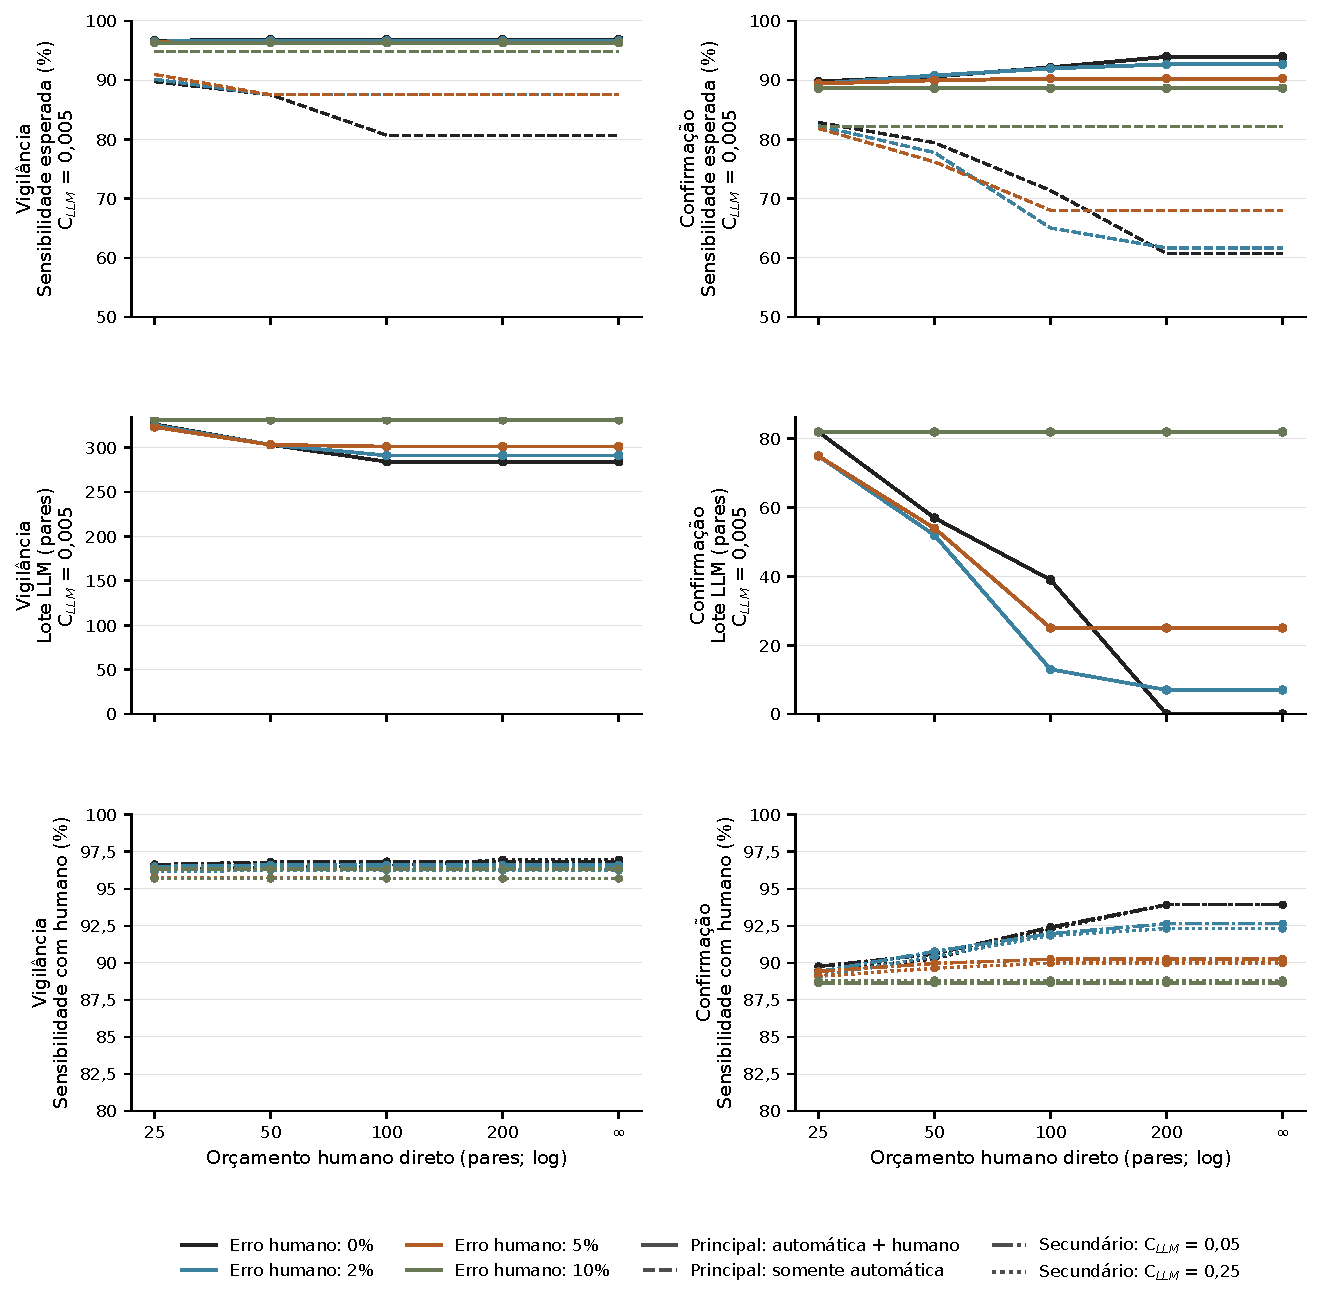
\includegraphics[width=\textwidth,height=0.67\textheight,keepaspectratio]{figures/fig_cap8_varredura_custos.pdf}
\caption{Sensibilidade esperada e volume de revisão segundo o orçamento humano direto, o custo relativo do LLM e a hipótese de erro humano, nos modos vigilância (esquerda) e confirmação (direita). As duas primeiras linhas de painéis (cenário principal) usam $C_{LLM}=0{,}005$: a primeira mostra a sensibilidade esperada, com humano (linha contínua) e somente automática (tracejada), e a segunda, o lote do LLM. A terceira linha (cenários secundários) mostra a sensibilidade esperada com humano para $C_{LLM}=0{,}05$ (traço e ponto) e $C_{LLM}=0{,}25$ (pontilhada). As cores representam hipóteses de erro humano, não proporções medidas; o eixo horizontal é logarítmico e $\infty$ indica orçamento ilimitado, não um limite de 400 pares. O limite direto exclui a carga humana de inconclusivos.}
\label{fig:cap8-varredura-custos}
\end{figure}

Com humanos ilimitados, passar de $C_{LLM}=0{,}25$ e erro humano nulo para $C_{LLM}=0{,}005$ e erro humano de 5,0\% alterou, na vigilância, o lote LLM de 212 para 347 pares, a carga humana total esperada de 218,5 para 98,8 e a sensibilidade esperada após revisão humana de 96,3\% para 95,1\%. Na confirmação, a mesma mudança fez o lote LLM passar de zero para 44 pares e os encaminhamentos diretos caírem de 229 para 121, com carga humana total esperada de 229,0 para 124,3 e sensibilidade esperada de 92,3\% para 87,7\%. A \textit{expected loss} total passou de 1.208,20 para 1.291,42 na vigilância e de 731,87 para 1.121,49 na confirmação, em revisões humanas equivalentes. A comparação altera ao mesmo tempo o custo do LLM e a hipótese de erro humano e não isola o efeito de cada um.

\subsection{Confirmação por restrição de falsos positivos na base inteira}
\label{sec:e4-np-confirmacao}

A minimização de custo não garante um limite predefinido de falsos positivos automáticos. A política denominada NP na implementação ordena os candidatos a vínculo por $p$ decrescente e escolhe o prefixo com maior número esperado de vínculos, sujeito a
\[
\sum_{i\in\mathcal{M}}(1-p_i)\leq\alpha\,|\mathcal{M}|,
\]
em que $\mathcal{M}$ inclui os vínculos das guardas e os demais vínculos automáticos. A restrição controla a fração esperada de falsos positivos entre as decisões de vínculo, e não $P(\texttt{MATCH}\mid\text{não par})$ do teste de Neyman e Pearson, sem implicar garantia frequentista.

Fora das guardas, exigiu-se $p\leq0{,}02$ para \texttt{NONMATCH} automático; o restante foi ao LLM apenas quando sua \textit{expected loss} era menor que a humana e havia orçamento, ou ao revisor humano. Capacidade humana insuficiente ou restrição incompatível com as guardas torna o cenário inviável, sem métricas iguais a zero.

Os alvos de 0,1\% e 0,2\% foram inviáveis com as guardas mantidas: embora os 63 vínculos automáticos não tivessem falsos positivos observados, a soma de $1-p$ foi de 0,67 falso positivo esperado, e mesmo com os 47 candidatos mais favoráveis ($p=1$) o limite mínimo foi de 0,61\%, entre 110 vínculos automáticos (Figura~\ref{fig:cap8-np-confirmacao}). O risco esperado não se substitui pela ausência de erro observado, e seu controle depende da calibração absoluta: a sobreconfiança das Seções~\ref{sec:e4-classificador-oof} e~\ref{sec:e4-calibracao-beta} pode subestimar $1-p$.

\begin{figure}[!htbp]
\centering
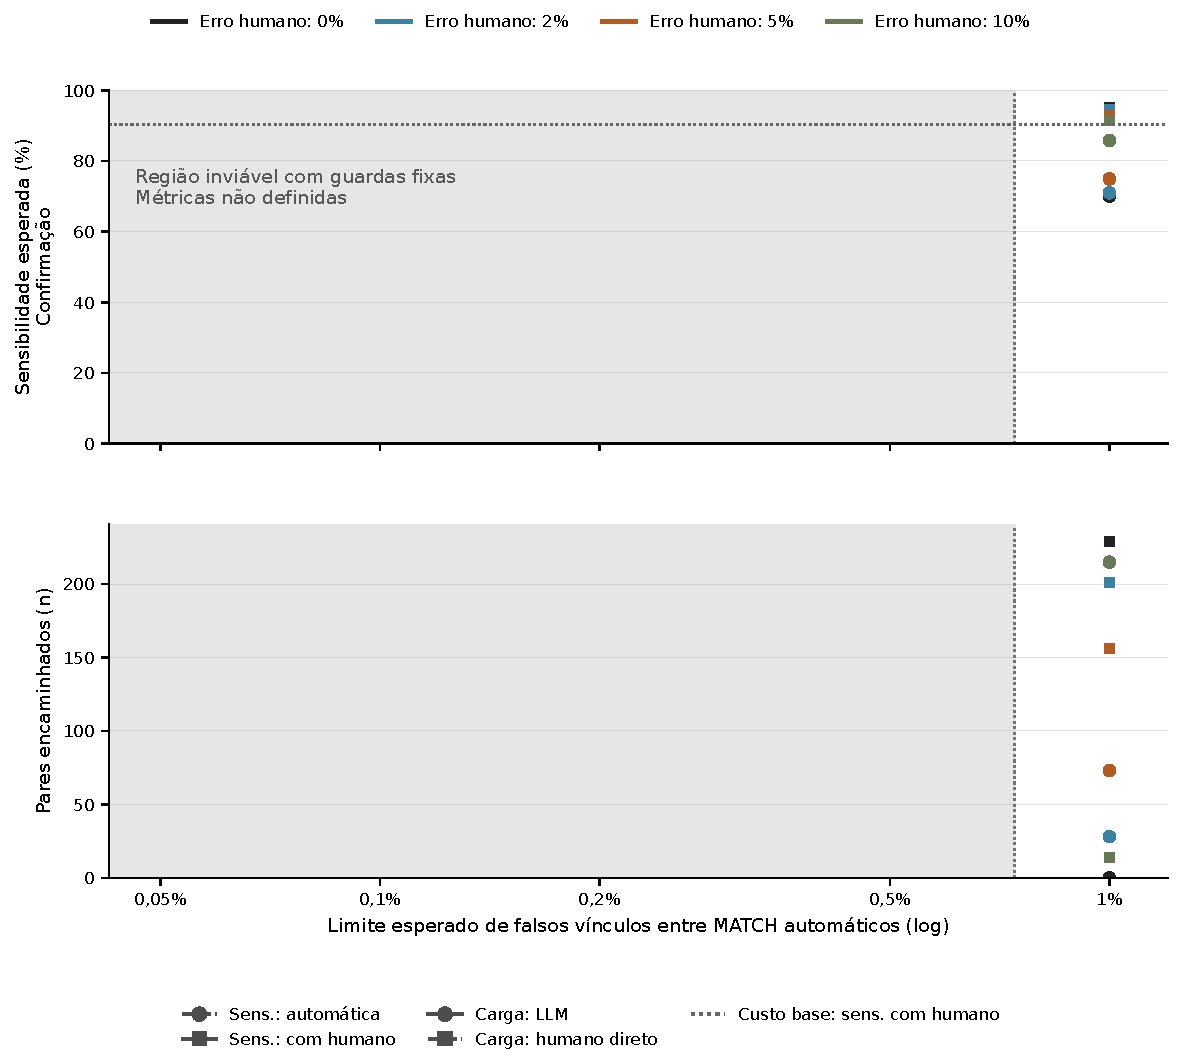
\includegraphics[width=\textwidth,height=0.60\textheight,keepaspectratio]{figures/fig_cap8_np_confirmacao.pdf}
\caption{Política por restrição na confirmação: sensibilidade esperada (superior) e encaminhamentos ao LLM e ao revisor humano direto (inferior), segundo o limite da fração esperada de falsos positivos entre os vínculos automáticos. As cores representam hipóteses de erro humano; a linha pontilhada é a sensibilidade com humano da política por custo; o sombreado marca limites inviáveis com as guardas. São projeções, não resultados observados.}
\label{fig:cap8-np-confirmacao}
\end{figure}

O limite de 1,0\% foi viável com orçamento humano ilimitado, mas exigiu mais revisão e maior \textit{expected loss} que a política por custo (Tabela~\ref{tab:cap8-np-confirmacao}): a sensibilidade esperada com revisão humana subiu de 87,7\% para 90,1\% e a carga humana total esperada passou de 124,3 para 247,0 pares. O limite incide só nos vínculos automáticos do motor, e não nos falsos positivos da cadeia, que incluem erros do LLM e do revisor humano.

\begin{table}[!htbp]
\centering
\caption{Confirmação por custo e por restrição NP (limite da fração esperada de falsos positivos entre os automáticos) de 1,0\%, com $C_{LLM}=0{,}005$, erro humano hipotético de 5,0\% e orçamento humano ilimitado. Os valores são expectativas, não resultados observados.}
\label{tab:cap8-np-confirmacao}
\begin{tabular}{lrr}
\hline
Indicador & Custo & NP 1,0\% \\
\hline
Pares selecionados para LLM & 44 & 108 \\
Encaminhamentos humanos diretos & 121 & 241 \\
Carga humana total esperada & 124,3 & 247,0 \\
Sensibilidade automática esperada (\%) & 55,7 & 62,7 \\
Sensibilidade esperada com humano (\%) & 87,7 & 90,1 \\
FP esperados nos vínculos automáticos, com guardas & 0,83 & 1,29 \\
FP esperados na cadeia completa & 2,88 & 10,96 \\
\textit{Expected loss} (revisões humanas equivalentes) & 1.121,49 & 1.859,28 \\
\hline
\end{tabular}
\end{table}

\section{Seleção e avaliação do revisor LLM}\label{sec:e4-ap-revisor}

Esta seção reúne a seleção do LLM no piloto, os experimentos de revisão assistida com dossiê completo, a replicação com revisores independentes, a ablação do dossiê, as reavaliações sem as saídas do motor e os custos do arranjo e da cascata.

\subsection{Seleção do modelo de linguagem}\label{sec:e4-selecao-llm}

A execução histórica do protocolo usou a API Fireworks AI, com temperatura zero e semente fixa (seed=43); o provedor não foi usado nas execuções posteriores, e seus resultados estão na Seção~\ref{sec:e4-llm-inicial}. Na v3, o carregador omitiu a política por faixa posterior à separadora do arquivo-base, embora a mensagem de usuário a solicitasse (Apêndice~\ref{sec:apendice-prompts}).

A escolha do modelo considerou a concordância com a referência operacional, o valor preditivo positivo (VPP), a sensibilidade, o F$_1$, a latência por par e a proporção de inconclusivos. O piloto avaliou 517 pares do lote selecionado pelo motor pela sequência operacional (\textit{pipeline}) v3 (Tabela~\ref{tab:cap8-llm-piloto}). Pela nota final do CdR, 341 dos 517 pares (66,0\%) situam-se abaixo da nota 5, fora da faixa intermediária da nota final $[5,9)$, que reúne 168 pares (32,5\%); o piloto não representa essa faixa. Cinco modelos foram testados com \texttt{temperature}=0, \texttt{max\_tokens}=4096, \texttt{top\_p}=1, \texttt{top\_k}=40 e penalidades nulas: Kimi~K2.5, GPT-4o, DeepSeek~V3.2, Qwen3-VL-30B (30 bilhões de parâmetros) e GLM-5. Kimi, DeepSeek, Qwen e GLM foram acessados pela Fireworks AI e GPT-4o, pela API da OpenAI (\path{scripts/pilot_c2_517.py}).

Esses parâmetros descrevem o piloto, não todos os revisores posteriores. Na replicação, DeepSeek V4.1 Flash utilizou \texttt{temperature}=0, \texttt{top\_p}=1, \texttt{top\_k}=1 e \texttt{max\_tokens}=800 por chamada, com raciocínio desligado (\path{thinking.type=disabled} e \path{reasoning_effort=none}); Kimi K3 utilizou os mesmos parâmetros de amostragem, \texttt{max\_\allowbreak tokens}=2500 e \path{reasoning_effort=low}. Os JSONs históricos em \path{data/sprint3b/} não preservam todos os parâmetros de geração, que constam dos \textit{scripts} \path{run_exp2_opencode_go.py} e \path{run_exp2_anthropic.py} \cite{Jardim2026phdrepo}.

\begin{table}[!ht]
\centering
\caption{Avaliação comparativa de modelos para revisão assistida ($n=517$ pares do lote selecionado pelo motor; intervalos de Wilson, 95\%).}
\label{tab:cap8-llm-piloto}
\resizebox{\textwidth}{!}{%
\begin{tabular}{|l|c|c|c|c|c|c|c|}
\hline
Modelo & Válidos$^a$ & Concordância (\%) & VPP & Sensibilidade & F$_1$ & Inconcl.\,(\%) & Latência (s/par) \\
\hline
Kimi K2.5      & 499 & 97,8\,[96,1;\,98,8] & 0,909 & 0,789 & \textbf{0,845} & 3,5  & 7,3 \\
\hline
GPT-4o         & 508 & 95,5\,[93,3;\,97,0] & 1,000 & 0,343 & 0,511          & 1,7  & 6,3 \\
\hline
DeepSeek V3.2  & 232 & 93,5\,[89,6;\,96,0] & 0,615 & 0,762 & 0,681          & 55,1 & 54,0 \\
\hline
Qwen3-VL-30B   & 509 & 94,9\,[92,6;\,96,5] & 1,000 & 0,333 & 0,500          & 1,6  & 7,5 \\
\hline
GLM-5           & 212 & 95,3\,[91,5;\,97,4] & 0,769 & 0,833 & 0,800          & 59,0 & 57,6 \\
\hline
\multicolumn{8}{l}{\footnotesize $^a$\,Pares com decisão \texttt{MATCH}/\texttt{NONMATCH}; excluídos os \texttt{UNSURE}.} \\
\end{tabular}%
}
\end{table}

A concordância exclui inconclusivos e tem denominadores de 212 a 509 (Tabela~\ref{tab:cap8-llm-piloto}), e a abstenção seletiva favorece a concordância entre os resolvidos. Para discriminar, com poder de 80\% (nível de significância de 5\%, teste bilateral, aproximação normal para duas proporções independentes), a concordância de 97,8\% do Kimi K2.5 de 94,3\%, diferença de 3,5 pontos percentuais, seriam necessários 485 pares por modelo; para uma diferença de 1,5 ponto percentual (97,8\% contra 96,3\%), 1.997 pares por modelo (\path{scripts/poder_amostral_piloto.py}).

GPT-4o e Qwen3-VL-30B tiveram VPP de 1,000 e sensibilidade baixa ($\approx$0,34), com omissão de pares verdadeiros; DeepSeek~V3.2 e GLM-5 tiveram mais de 55\% de inconclusivos e latência superior a 54~s/par. Kimi K2.5 teve o maior F$_1$ pontual (0,845), com 3,5\% de inconclusivos e latência de 7,3~s/par, sem superioridade demonstrada em concordância global. Entre os 499 pares com decisão válida, o Kimi~K2.5 teve 30 verdadeiros positivos, 3 falsos positivos, 8 falsos negativos e 458 verdadeiros negativos. GPT-4o e Qwen3-VL-30B não produziram falsos positivos, mas omitiram, respectivamente, 23 e 26 pares verdadeiros, padrão que tenderia a subestimar a mortalidade por tuberculose na vigilância. DeepSeek~V3.2 e GLM-5 tiveram sensibilidade de 76,2\% e 83,3\%, mas a proporção elevada de inconclusivos reduz o denominador efetivo a menos da metade da amostra.

O Kimi~K2.5 usou o árbitro em 14 casos (2,7\%), e DeepSeek~V3.2 e GLM-5, em 213 (41,2\%) e 155 (30,0\%) pares, com latências superiores a 54~s/par. A indução de cadeias de raciocínio (\textit{chain-of-thought}) foi proposta como técnica de elaboração de respostas por etapas \cite{Wei2022chainofthought}; uma hipótese, não testada no piloto, é que a cadeia estendida tenha levado esses modelos a sinalizar incerteza com mais frequência, e a latência maior não veio acompanhada de concordância maior que a do Kimi~K2.5. Os intervalos de Wilson para a concordância sobrepõem-se entre os cinco modelos, o que impede rejeitar igualdade ao nível de 95\% de confiança, mas o F$_1$ varia de 0,500 (Qwen3-VL-30B) a 0,845 (Kimi~K2.5). A concordância global é dominada pelos verdadeiros negativos, enquanto o F$_1$ pondera a detecção da classe minoritária (476 não pares contra 41 pares); sob forte desbalanceamento, as métricas devem ser reportadas por classe.

\subsection{Experimento 2: desempenho da revisão assistida}
\label{sec:e4-exp2}

O resultado histórico do Experimento 2 corresponde à execução de fevereiro de 2026 com Kimi K2.5, instruções v3 e dossiê completo, incluindo as saídas decisórias do motor. O lote de 1.410 potenciais pares foi selecionado pela política v3, não corresponde à totalidade da faixa intermediária da nota final e inclui 22 pares com nota final do CdR $v\geq9$. A Tabela~\ref{tab:cap8-revisao-desempenho} apresenta a matriz reconstruída contra a referência operacional, separando esse estrato dos pares com $v<9$, para não atribuir à região de maior ambiguidade a sensibilidade obtida entre os pares de nota final elevada \cite{Jardim2026phdrepo}.

\begin{table}[!ht]
\centering
\caption{Resultado histórico observado do Kimi K2.5 no Experimento 2 (Exp2, revisão assistida), por nota final $v$ do Comparador de Registros (CdR), com dossiê completo (incluindo as saídas decisórias do motor) e instruções v3 (versão histórica que solicita essas saídas), em fevereiro de 2026.}
\label{tab:cap8-revisao-desempenho}
\begin{tabular}{lrrrrrrr}
\hline
Nota final & $N$ & VP & FP & FN & VN & Inconcl. & Pares verd. inconcl. \\
\hline
$v<9$ & 1.388 & 57 & 6 & 19 & 1.265 & 41 & 6 \\
$v\geq9$ & 22 & 22 & 0 & 0 & 0 & 0 & 0 \\
Total & 1.410 & 79 & 6 & 19 & 1.265 & 41 & 6 \\
\hline
\end{tabular}%
\par\smallskip
\parbox{\linewidth}{\footnotesize VP: verdadeiros positivos; FP: falsos positivos; FN: falsos negativos; VN: verdadeiros negativos. Os inconclusivos são apresentados separadamente, sem integrar a matriz dos resolvidos. Fonte: \texttt{data/exp2\_gabarito\_reconstruido.csv} e \texttt{data/exp2\_reruns\_por\_banda.csv} \cite{Jardim2026phdrepo}.}
\end{table}

Os valores foram reconstruídos por \path{scripts/reconstruir_gabarito_exp2.py}, por cruzamento com a referência operacional pelo \texttt{pair\_id}, pseudônimo determinístico calculado pelo SHA-256 da concatenação de \texttt{COMPREC}, \texttt{REFREC} e \texttt{PASSO}, sem sal e truncado em 16 caracteres hexadecimais. Por ser recalculável por quem dispõe dos identificadores internos, não garante anonimização irreversível; a exportação restrita com HMAC-SHA256, para novas exportações, está na Seção~\ref{sec:export-restrita}. Entre os 1.369 pares resolvidos, a sensibilidade foi de 80,6\% e o VPP de 92,9\%; no estrato $v<9$, a sensibilidade foi de 75,0\%, contra 100,0\% nos 22 pares verdadeiros com $v\geq9$. Dos 104 pares verdadeiros do lote, 19 receberam \texttt{NONMATCH} e 6 ficaram entre os 41 inconclusivos. Como o dossiê continha as saídas do motor, a interpretação desse resultado depende do exame de ancoragem da Seção~\ref{sec:e4-ablacao-dossie} \cite{Jardim2026phdrepo}.

\subsection{Revisão assistida por modelo de linguagem: execução inicial}\label{sec:e4-llm-inicial}

Na política v3, o lote de 1.410 pares da vigilância foi selecionado pelo valor esperado da revisão (EVR), pelos limites automáticos de probabilidade e pela regra de homonímia, com as prioridades da Seção~\ref{sec:e4-motor-politica}, e não por consenso entre classificadores. Nesse estrato, um modelo de linguagem de grande porte (LLM) atua como revisor complementar sobre dossiês estruturados, segundo o protocolo de dois agentes com árbitro da Seção~\ref{sec:e4-protocolo-llm}. O consenso entre os dois agentes primários alcançou 97{,}2\% na vigilância e 94{,}7\% na confirmação, o que mede concordância entre agentes, não acerto frente à referência operacional.

% Gerada por scripts/banca_c_agregados.py; não editar manualmente.
\begin{table}[htbp]
\centering
\small
\caption{Matrizes de confusão da execução anterior de Kimi K2.5, por modo de operação (15 de fevereiro de 2026).}
\label{tab:qw2-confusion}
\begin{tabular}{llrrrl}
\toprule
Modo & Classe real & MATCH & NONMATCH & Total & Protocolo \\
\midrule
Vigil\^ancia & Par verdadeiro & 72 & 32 & 104 & consenso: 1.371; \'arbitro: 39 \\
Vigil\^ancia & N\~ao par & 6 & 1.300 & 1.306 & -- \\ \midrule
Confirma\c{c}\~ao & Par verdadeiro & 91 & 10 & 101 & consenso: 412; \'arbitro: 23 \\
Confirma\c{c}\~ao & N\~ao par & 3 & 331 & 334 & -- \\
\bottomrule
\end{tabular}
\par\smallskip\parbox{\linewidth}{\footnotesize Fonte: \path{data/qw2_kimi_agregado.csv}, gerado de JSONs privados por \path{scripts/banca_c_agregados.py}, com hash de cada fonte e sem dados por par. A vigilância é execução anterior, distinta da matriz reconstruída da Tabela~\ref{tab:cap8-revisao-desempenho}. Comparações entre revisores: Tabela~\ref{tab:cap8-reruns}.}
\end{table}


Os resultados indicam desempenho assimétrico entre os modos (Tabela~\ref{tab:qw2-confusion}). Na vigilância, o Kimi K2.5 revisou 1.410 pares e obteve VPP de 0{,}923 com sensibilidade de 0{,}692, o que resulta em $F_1 = 0{,}791$, em execução anterior do mesmo protocolo, de 15 de fevereiro de 2026, registrada em \path{data/qw2/qw2_vigilancia_kimi.json} e sintetizada, sem \texttt{pair\_id}, respostas individuais ou texto livre, em \path{data/qw2_kimi_agregado.csv}, gerado por \path{scripts/banca_c_agregados.py}. Essa execução difere da matriz reconstruída a partir de \path{data/sprint3b/exp2_llm_sync_vigilancia.json}, apresentada na Tabela~\ref{tab:cap8-revisao-desempenho}. A Tabela~\ref{tab:cap8-reruns} é a referência para comparar revisores e reavaliações. A especificidade foi alta ($0{,}995$), mas 32 pares verdadeiros receberam \texttt{NONMATCH}, perda de 30{,}8\% dos positivos nesse estrato residual, que deve ser lida à luz da ancoragem nas saídas do motor e não atribuída apenas à ausência de campos textuais brutos.

No modo confirmação, sobre 435 pares, o VPP atinge 0{,}968 e a sensibilidade sobe para 0{,}901, elevando o $F_1$ para 0{,}933. A prevalência de pares verdadeiros nesse modo (23{,}2\%) é maior que na vigilância (7{,}4\%); o VPP depende dessa prevalência, e os lotes diferem em composição, o que impede atribuir a diferença entre modos apenas ao revisor.

% Gerada por scripts/banca_c_agregados.py; não editar manualmente.
\begin{table}[htbp]
\centering
\small
\caption{Desempenho de Kimi K2.5 na execução anterior da revisão assistida de pares residuais, por modo de operação.}
\label{tab:qw2-llm-comparison}
\begin{tabular}{lrrrrrr}
\toprule
Modo & $n$ & Precis\~ao & Sensibilidade & $F_1$ & Especif. & Acur\'acia \\
\midrule
Vigil\^ancia & 1.410 & 0,923 & 0,692 & 0,791 & 0,995 & 0,973 \\
Confirma\c{c}\~ao & 435 & 0,968 & 0,901 & 0,933 & 0,991 & 0,970 \\
\bottomrule
\end{tabular}
\par\smallskip\parbox{\linewidth}{\footnotesize Fonte: \path{data/qw2_kimi_agregado.csv}, gerado de JSONs privados por \path{scripts/banca_c_agregados.py}, com hash de cada fonte e sem dados por par. A vigilância é execução anterior, distinta da matriz reconstruída da Tabela~\ref{tab:cap8-revisao-desempenho}. Comparações entre revisores: Tabela~\ref{tab:cap8-reruns}.}
\end{table}


A Tabela~\ref{tab:qw2-llm-comparison} sintetiza as métricas nos dois modos. A diferença de sensibilidade ($0{,}692$ \textit{versus} $0{,}901$) descreve lotes de composição distinta e dossiês com saídas do motor (Seção~\ref{sec:e4-ablacao-dossie}); as chamadas são individuais, sem informar a prevalência do lote ao modelo. Esses achados sugeriram adequação do LLM à confirmação, mas não se mantiveram na cascata sobre a base inteira (Seção~\ref{sec:e4-cascata}), na qual o LLM recebeu poucos potenciais pares da confirmação e a revisão humana concentrou o esforço. Para a vigilância, a perda de sensibilidade aponta para o encaminhamento ao revisor humano da quarta ação da política v3.1 (Seção~\ref{sec:e4-politica-v31}) ou para a inclusão de campos textuais no dossiê.

\subsection{Replicação da revisão assistida com revisores independentes}
\label{sec:e4-revisores}

A replicação com dossiê completo e instruções v3 utilizou DeepSeek V4.1 Flash, via OpenCode Go, com raciocínio desligado e temperatura zero, e Claude Haiku 5.5, via API da Anthropic, sem parâmetro de temperatura. No modo confirmação, Kimi K3, com esforço de raciocínio baixo, completou apenas 343 dos 435 pares, por esgotamento de cota. Os modelos receberam o mesmo lote e o protocolo de dois agentes com árbitro; a denominação de revisores independentes refere-se às instâncias e aos fornecedores, embora o dossiê contivesse informação decisória prévia. A Tabela~\ref{tab:cap8-revisores} reestratifica os resultados por nota final $v<9$ e $v\geq9$. O resultado de Kimi K2.5 na confirmação provém da fonte alternativa QW2 (registro das execuções de revisão por modelo de linguagem) e é identificado na Tabela~\ref{tab:cap8-reruns}; a equivalência de protocolo com a execução histórica de vigilância ainda não foi verificada \cite{Jardim2026phdrepo}.

% Fonte: data/exp2_reruns_por_banda.csv, estrato limiar_9, dossiê completo/v3.
\begin{table}[!htbp]
\centering
\caption{Resultados observados dos revisores com dossiê completo e instruções v3, estratificados pela nota final do Comparador de Registros (CdR), $v$.}
\label{tab:cap8-revisores}
\footnotesize
\resizebox{\linewidth}{!}{%
\begin{tabular}{llrrrrrrr}
\hline
Revisor & Nota & $N$ & VP & FP & FN & VN & Inconcl. (pares verdadeiros) & Sens. (\%) \\
\hline
\multicolumn{9}{l}{\textbf{Vigilância}} \\
Kimi K2.5 & $v<9$ & 1.388 & 57 & 6 & 19 & 1.265 & 41 (6) & 75,0 \\
 & $v\geq9$ & 22 & 22 & 0 & 0 & 0 & 0 (0) & 100,0 \\
DeepSeek V4.1 Flash & $v<9$ & 1.388 & 27 & 3 & 42 & 1.256 & 60 (13) & 39,1 \\
 & $v\geq9$ & 22 & 22 & 0 & 0 & 0 & 0 (0) & 100,0 \\
Claude Haiku 5.5 & $v<9$ & 1.388 & 16 & 0 & 10 & 1.103 & 259 (56) & 61,5 \\
 & $v\geq9$ & 22 & 19 & 0 & 0 & 0 & 3 (3) & 100,0 \\
Levanto Sage 2 & $v<9$ & 1.388 & 36 & 9 & 20 & 1.224 & 99 (26) & 64,3 \\
 & $v\geq9$ & 22 & 13 & 0 & 1 & 0 & 8 (8) & 92,9 \\
\hline
\multicolumn{9}{l}{\textbf{Confirmação}} \\
DeepSeek V4.1 Flash & $v<9$ & 377 & 12 & 1 & 8 & 287 & 69 (24) & 60,0 \\
 & $v\geq9$ & 58 & 57 & 1 & 0 & 0 & 0 (0) & 100,0 \\
Claude Haiku 5.5 & $v<9$ & 377 & 6 & 0 & 5 & 203 & 163 (33) & 54,5 \\
 & $v\geq9$ & 58 & 49 & 1 & 0 & 0 & 8 (8) & 100,0 \\
Kimi K3 (parcial) & $v<9$ & 295 & 15 & 2 & 16 & 248 & 14 (9) & 48,4 \\
 & $v\geq9$ & 48 & 42 & 1 & 0 & 0 & 5 (5) & 100,0 \\
\hline
\end{tabular}%
}
\par\smallskip
\parbox{\linewidth}{\footnotesize VP: verdadeiros positivos; FP: falsos positivos; FN: falsos negativos; VN: verdadeiros negativos. Sensibilidade entre resolvidos: $VP/(VP+FN)$; inconclusivos não são acertos. Kimi K3: 343 respostas em 435 pares, sem imputação dos 92 ausentes. Levanto Sage 2 utiliza uma escolha por par, não dois agentes e árbitro; a comparação não isola o efeito do modelo. Fonte: \texttt{data/exp2\_reruns\_por\_banda.csv} \cite{Jardim2026phdrepo}.}
\par\footnotesize Dossiê completo: inclui as saídas decisórias do motor. Instruções v3: solicitam essas saídas. CdR: Comparador de Registros; $v$: sua nota final.
\end{table}


Com \texttt{UNSURE} como terceira categoria, o kappa de Cohen \cite{McHugh2012kappa} entre Kimi K2.5 e DeepSeek V4.1 Flash foi de 0,745 na vigilância; entre Kimi K2.5 e Claude Haiku 5.5, de 0,426; e entre DeepSeek e Haiku, de 0,442. Excluindo os inconclusivos de qualquer revisor, os valores foram, respectivamente, 0,794, 0,985 e 1,000. Na confirmação, DeepSeek e Haiku apresentaram kappa de 0,495 com inconclusivos e 1,000 sem eles. Os denominadores variam com a disponibilidade de respostas e a exclusão de inconclusivos (\texttt{data/exp2\_kappas\_revisores.csv}), e a concordância perfeita no subconjunto resolvido não representa concordância em toda a coorte.

Na vigilância, o DeepSeek V4.1 Flash reconheceu os 22 pares verdadeiros com $v\geq9$, mas teve sensibilidade de 39,1\% nos resolvidos com $v<9$; o Claude Haiku 5.5 teve, nesse estrato, sensibilidade de 61,5\%, com 259 inconclusivos. Os erros compartilhados motivaram a ablação do dossiê, e não foram atribuídos apenas à insuficiência dos campos de identificação.

Foi testado também o Levanto Sage 2 (\texttt{levanto-sage-2}), modelo de decisão que escolhe entre aceitar como vínculo e rejeitar, com possibilidade de abstenção, em uma decisão por par e sem o protocolo de dois agentes e árbitro. Na vigilância, com as saídas do motor, a especificidade foi de 99,3\% e a sensibilidade de 70,0\% entre os resolvidos; sem elas, houve 164 falsos positivos e 446 inconclusivos em 1.410 pares, com AUC de 0,82 para a probabilidade de par verdadeiro, calculada com \texttt{probabilities[match]} e não com a confiança na escolha devolvida. Os resultados constam de \texttt{data/exp2\_sage\_resumo.csv} e \texttt{data/exp2\_sage\_relatorio.md}; diferenças de protocolo e execuções únicas impedem atribuir o contraste apenas ao modelo \cite{Jardim2026phdrepo}.

\subsection{Ablação do dossiê: mudanças de decisão sem as saídas do motor}
\label{sec:e4-ablacao-dossie}

Os falsos negativos compartilhados pelos três revisores que receberam o mesmo dossiê motivaram uma hipótese distinta da insuficiência da evidência de identificação: a apresentação das saídas do motor poderia induzir ancoragem na decisão previamente calculada, reduzindo a independência da revisão. O grupo \texttt{model\_outputs} reúne \texttt{p\_cal}, \texttt{base\_choice}, \texttt{band}, \texttt{evr}, \texttt{guardrail} e \texttt{guardrail\_reason}. Na calibração histórica, \texttt{p\_cal} é função monótona da nota final do comparador, e os demais campos também podem transmitir informação sobre a probabilidade ou a decisão do motor.

Foram selecionados 18 pares verdadeiros que, na vigilância, receberam \texttt{NONMATCH} de pelo menos dois dos três revisores originais; nove foram rejeitados pelos três. Cada par foi submetido ao controle com dossiê completo e ao braço \texttt{sem\_pcal}, em que a função \texttt{ablate()} retira o grupo \texttt{model\_outputs} e preserva subescores, nota final e as Medidas Contínuas de Diferença de Datas de nascimento, MACD (\path{scripts/run_exp2_ablacao_dossie.py}). Mantêm-se o prompt original e o protocolo de dois agentes com árbitro. A busca nos cinco originais locais, nas seis coortes históricas, inclusive \path{data/sprint3b/anthropic_sem_mo_v4/}, e no histórico do executor não recuperou versão ou hash que certifique o prompt dos braços selecionados; as coortes completas v4 registram versão e hash, sem estabelecer identidade com os braços de 18 (\path{data/sprint3b/ablacao/ablacao_dossie_proveniencia.json}). DeepSeek V4.1 Flash e Claude Haiku 5.5 completaram ambos; Kimi K3 participou de sondagem em três pares, sem integrar a inferência pareada. As contagens estão em \path{data/ablacao_dossie_agregado.json} e nos agregados \path{data/sprint3b/ablacao/*_agregado.json}, sem identificadores individuais \cite{Jardim2026phdrepo}.

A comparação pareada usou o teste de McNemar exato bilateral, com a decisão \texttt{MATCH} em oposição às demais como desfecho primário e sem ajuste de multiplicidade. A passagem de \texttt{NONMATCH} para \texttt{UNSURE} foi contabilizada separadamente, pois retira a rejeição explícita do par verdadeiro, mas não é reconhecimento correto. A Tabela~\ref{tab:cap8-ablacao-dossie} distingue essas transições e apresenta a concordância entre o controle e a execução original, que avalia repetibilidade neste subconjunto, não acurácia no lote completo.

% Fontes: data/ablacao_dossie_relatorio.md, data/ablacao_dossie_agregado.json
% e data/sprint3b/ablacao/resumo.json.
\begin{table}[!ht]
\centering
\footnotesize
\caption{Ablação conjunta das saídas do motor no dossiê de revisão, em 18 pares verdadeiros selecionados por falso negativo compartilhado no modo vigilância.}
\label{tab:cap8-ablacao-dossie}
\resizebox{\linewidth}{!}{%
\begin{tabular}{lccrrrc}
\toprule
Modelo & \shortstack{Controle\\M/U/N} & \shortstack{Ablação\\M/U/N} & \shortstack{FN para\\MATCH} & \shortstack{FN para\\UNSURE} & \shortstack{McNemar\\$p$} & \shortstack{Controle =\\original} \\
\midrule
DeepSeek V4.1 Flash & 0/0/18 & 9/9/0 & 9 & 9 & 0,004 & 18/18 \\
Claude Haiku 5.5 & 0/9/9 & 7/11/0 & 2 & 7 & 0,016 & 13/18 \\
\bottomrule
\end{tabular}%
}
\par\smallskip
\parbox{\linewidth}{\footnotesize M: \texttt{MATCH} (vínculo); U: \texttt{UNSURE} (inconclusivo); N: \texttt{NONMATCH} (não aceito como vínculo). FN: falsos negativos do braço controle, não da execução original. Ablação: retirada de todo o grupo \texttt{model\_outputs}. McNemar exato bilateral para \texttt{MATCH} versus demais decisões, sem ajuste de multiplicidade. A mudança para \texttt{UNSURE} não constitui reconhecimento correto do vínculo. Fonte: \texttt{data/sprint3b/ablacao/resumo.json} \cite{Jardim2026phdrepo}.}
\par\footnotesize Ablação: retirada conjunta das saídas decisórias do motor do dossiê, documento estruturado com os subescores disponíveis para a revisão.
\end{table}


Sem as saídas do motor, nenhum dos 18 pares verdadeiros foi rejeitado por qualquer dos dois modelos. No DeepSeek V4.1 Flash, os 18 falsos negativos do controle se distribuíram igualmente entre \texttt{MATCH} e \texttt{UNSURE} após a ablação; no Claude Haiku 5.5, dos 9 falsos negativos do controle, 2 passaram a \texttt{MATCH} e 7 a \texttt{UNSURE}. As sete decisões \texttt{MATCH} do Claude Haiku 5.5 incluem ainda cinco pares inconclusivos no controle, razão pela qual o teste de McNemar para \texttt{MATCH} não se restringe às duas reversões. O controle reproduziu todas as decisões originais do DeepSeek V4.1 Flash, mas apenas 13 das 18 do Claude Haiku 5.5, o que documenta variabilidade entre execuções deste último, cuja API não recebeu parâmetro de temperatura.

A avaliação compreende apenas 18 pares, selecionados por erro compartilhado, e não estima o desempenho da ablação no conjunto dos potenciais pares nem o efeito sobre falsos positivos. O controle reproduz esse viés de seleção e não é amostra independente. A comparação informa a mudança de decisão neste subconjunto condicionado ao erro, com variabilidade entre execuções no Claude Haiku 5.5, e não autoriza generalizar a ausência de rejeições aos demais pares verdadeiros.

\subsection{Reavaliação sem as saídas do motor: detalhe}\label{sec:e4-ap-reavaliacao}

O protocolo de dois agentes e árbitro e o esquema de resposta foram preservados. A versão e o SHA-256 do arquivo completo de instruções v4 foram registrados nos metadados (\texttt{gzcmd/M4\_prompt\_v4.md}), com \textit{checkpoints} separados por versão, e as mesmas instruções valeram para as coortes de vigilância e confirmação selecionadas pelo motor. A Tabela~\ref{tab:cap8-reruns} reúne resultados históricos e reavaliações, distinguindo dossiê, versão das instruções e execução parcial \cite{Jardim2026phdrepo}.

% Gerada por scripts/avaliar_reruns_exp2.py; fonte: data/exp2_reruns_resumo.csv.
\begin{table}[!ht]
\centering
\footnotesize
\caption{Avaliação dos revisores no Experimento 2 (revisão assistida por LLM), segundo o dossiê (completo ou sem as saídas do motor, MO) e as instruções (v3, que solicitam essas saídas, ou v4, que não as solicitam), eixos independentes: há combinações como \textit{Sem MO/v3}.}
\label{tab:cap8-reruns}
\resizebox{\linewidth}{!}{%
\begin{tabular}{llrrrrrrr}
\toprule
Modelo & Dossiê/prompt & VP & FP & FN & UNSURE & Sens. (\%) & Espec. (\%) & UNSURE (\%) \\
\midrule
\multicolumn{9}{l}{\textbf{Vigilância}} \\
Kimi K2.5 & Completo/v3 & 79 & 6 & 19 & 41 & 80,6 (71,7; 87,2) & 99,5 (99,0; 99,8) & 2,9 \\
DeepSeek V4.1 Flash & Completo/v3 & 49 & 3 & 42 & 60 & 53,8 (43,7; 63,7) & 99,8 (99,3; 99,9) & 4,3 \\
Claude Haiku 5.5 & Completo/v3 & 35 & 0 & 10 & 262 & 77,8 (63,7; 87,5) & 100,0 (99,7; 100,0) & 18,6 \\
Levanto Sage 2 & Completo/v3 & 49 & 9 & 21 & 107 & 70,0 (58,5; 79,5) & 99,3 (98,6; 99,6) & 7,6 \\
Claude Haiku 5.5 & Sem MO/v3 & 67 & 6 & 2 & 1.258 & 97,1 (90,0; 99,2) & 92,8 (85,1; 96,6) & 89,2 \\
DeepSeek V4.1 Flash & Sem MO/v3 & 89 & 67 & 0 & 1.216 & 100,0 (95,9; 100,0) & 36,2 (27,6; 45,7) & 86,2 \\
Levanto Sage 2 & Sem MO/v3 & 65 & 164 & 16 & 446 & 80,2 (70,3; 87,5) & 81,4 (78,7; 83,9) & 31,6 \\
Claude Haiku 5.5 & Sem MO/v4 & 73 & 34 & 19 & 61 & 79,3 (70,0; 86,4) & 97,3 (96,2; 98,1) & 4,3 \\
Claude Sonnet 5.5 & Sem MO/v4 & 82 & 52 & 12 & 164 & 87,2 (79,0; 92,5) & 95,5 (94,1; 96,5) & 11,6 \\
DeepSeek V4.1 Flash & Sem MO/v4 & 89 & 268 & 0 & 1.053 & 100,0 (95,9; 100,0) & 0,0 (0,0; 1,4) & 74,7 \\
Claude Haiku 5.5 & Sem MO/v4 (lote por linha) & 17 & 8 & 2 & 26 & 89,5 (68,6; 97,1) & 95,1 (90,7; 97,5) & 12,4 \\
Claude Haiku 5.5 & Sem MO/v4 (lote REFREC) & 13 & 7 & 2 & 9 & 86,7 (62,1; 96,3) & 94,7 (89,4; 97,4) & 5,8 \\
\midrule
\multicolumn{9}{l}{\textbf{Confirmação}} \\
Kimi K2.5 & Completo/v3 & 91 & 3 & 10 & 0 & 90,1 (82,7; 94,5) & 99,1 (97,4; 99,7) & 0,0 \\
DeepSeek V4.1 Flash & Completo/v3 & 69 & 2 & 8 & 69 & 89,6 (80,8; 94,6) & 99,3 (97,5; 99,8) & 15,9 \\
Claude Haiku 5.5 & Completo/v3 & 55 & 1 & 5 & 171 & 91,7 (81,9; 96,4) & 99,5 (97,3; 99,9) & 39,3 \\
Kimi K3\textsuperscript{*} & Completo/v3 & 57 & 3 & 16 & 19 & 78,1 (67,3; 86,0) & 98,8 (96,5; 99,6) & 5,5 \\
Claude Haiku 5.5 & Sem MO/v3 & 72 & 3 & 0 & 347 & 100,0 (94,9; 100,0) & 81,2 (57,0; 93,4) & 79,8 \\
DeepSeek V4.1 Flash & Sem MO/v3 & 86 & 25 & 0 & 319 & 100,0 (95,7; 100,0) & 16,7 (7,3; 33,6) & 73,3 \\
Levanto Sage 2 & Sem MO/v3 & 38 & 7 & 50 & 38 & 43,2 (33,3; 53,6) & 97,7 (95,4; 98,9) & 8,7 \\
Claude Haiku 5.5 & Sem MO/v4 & 64 & 6 & 20 & 25 & 76,2 (66,1; 84,0) & 98,2 (96,0; 99,2) & 5,7 \\
Claude Sonnet 5.5 & Sem MO/v4 & 73 & 6 & 16 & 56 & 82,0 (72,8; 88,6) & 97,9 (95,6; 99,0) & 12,9 \\
DeepSeek V4.1 Flash & Sem MO/v4 & 87 & 97 & 0 & 251 & 100,0 (95,8; 100,0) & 0,0 (0,0; 3,8) & 57,7 \\
Claude Haiku 5.5 & Sem MO/v4 (lote por linha) & 2 & 0 & 1 & 1 & 66,7 (20,8; 93,9) & 100,0 (43,9; 100,0) & 14,3 \\
Claude Haiku 5.5 & Sem MO/v4 (lote REFREC) & 11 & 0 & 1 & 0 & 91,7 (64,6; 98,5) & 100,0 (56,6; 100,0) & 0,0 \\
\bottomrule
\end{tabular}%
}
\par\smallskip
\parbox{\linewidth}{\footnotesize VP: verdadeiros positivos; FP: falsos positivos; FN: falsos negativos. MO: bloco de saídas decisórias do motor. Sensibilidade e especificidade excluem \texttt{UNSURE}; a fração de \texttt{UNSURE} usa todas as respostas. NA indica denominador zero. O encaminhamento ao revisor humano não constitui acerto observado. Sensibilidade e especificidade apresentam IC de 95\% de Wilson entre parênteses; análises pareadas constam nos CSVs agregados. A confirmação de Kimi K2.5 utiliza a fonte alternativa QW2, sem pressupor equivalência de protocolo. As diferenças entre execuções não identificam isoladamente efeito causal do prompt. Claude Sonnet 5.5 (US\$ 2 e US\$ 10 por milhão de tokens de entrada e de saída, vinte vezes a tarifa do Claude Haiku 5.5) foi avaliado apenas com dossiê sem as saídas do motor e instruções v4, nas mesmas coortes do Haiku, e não alimenta as proporções da política (fonte: \texttt{data/exp2\_sonnet\_v4\_resumo.csv}). Lotes complementares são apresentados separadamente, com seleção distinta da coorte histórica; não constituem braços pareados adicionais. Fonte: artefatos do Exp2 \cite{Jardim2026phdrepo}.}
\par\smallskip
\parbox{\linewidth}{\footnotesize\textsuperscript{*} Execuções parciais, respostas disponíveis/coorte esperada: Kimi K3 (confirmacao, completo/v3): 343/435. Pares sem resposta não são classificados como \texttt{UNSURE}.}
\par\footnotesize REFREC identifica o registro do SIM. QW2: registro das execuções de revisão por modelo de linguagem.
\end{table}


O Claude Sonnet 5.5, com o mesmo dossiê sem as saídas do motor e instruções v4, foi avaliado nas mesmas coortes, a US\$~2 e US\$~10 por milhão de \textit{tokens} de entrada e de saída, vinte vezes a tarifa do Claude Haiku 5.5; suas respostas não alimentam as proporções da política, definidas apenas pelo Haiku. Na vigilância, observaram-se 82 verdadeiros positivos, 52 falsos positivos, 12 falsos negativos e 164 inconclusivos (11,6\%), com sensibilidade de 87,2\% e especificidade de 95,5\% entre os resolvidos; na confirmação, 73, 6, 16 e 56 inconclusivos (12,9\%), com sensibilidade de 82,0\% e especificidade de 97,9\%, e os intervalos de Wilson constam da tabela anterior. Pelo critério de acerto estrito, o Haiku acertou e o Sonnet errou em 137 pares da vigilância, contra 23 no sentido inverso (McNemar exato, $p<0{,}0001$), e em 41 pares da confirmação, contra 14 ($p=0{,}0004$); a discordância concentrou-se na faixa da nota final $[7,8)$, com 101 dos 137 pares na vigilância e 33 dos 41 na confirmação. O custo estimado das execuções do Sonnet foi de aproximadamente US\$~76 (\path{data/exp2_sonnet_v4_resumo.csv} e \path{data/exp2_sonnet_v4_relatorio.md}) \cite{Jardim2026phdrepo}.

Na cascata v3.1 com Sonnet como revisor, mantidos o lote e as proporções do Haiku, a cadeia aceitou 196 pares verdadeiros na vigilância, com 35 falsos positivos, perdeu 12 e encaminhou 134 pares ao humano, com sensibilidade automática de 79,4\% e, sob erro humano de 5\%, de 94,4\%; na confirmação, aceitou 136 pares verdadeiros, sem falso positivo, perdeu 27 e encaminhou 129 pares, com 55,1\% e 87,4\% (\path{data/funil_sonnet_v4_cascata.csv}). A cadeia com Sonnet encaminhou mais pares ao humano que a cadeia com Haiku (134 contra 111 e 129 contra 127); a comparação das aceitações está no corpo do capítulo.

Na comparação pareada de Claude Haiku 5.5 com instruções v3 e dossiê completo e Claude Haiku 5.5 com instruções v4 e sem as saídas do motor, os inconclusivos passaram de 262 para 61 na vigilância (18,6\% para 4,3\%). Houve 223 transições de ausência de acerto estrito para acerto e 65 no sentido inverso, com $p=1{,}97\times10^{-21}$ no teste de McNemar exato bilateral. Na confirmação, as transições foram 147 e 21, respectivamente ($p=1{,}78\times10^{-24}$). O acerto estrito exige decisão concordante com a referência operacional, sem contar inconclusivo como acerto; os valores de \texttt{data/exp2\_reruns\_pareado.csv} não isolam o efeito causal das instruções, pois também mudam o dossiê e o momento da execução, sem ajuste de multiplicidade.

Nas execuções sem as saídas do motor, o DeepSeek V4.1 Flash não apresentou falsos negativos explícitos em nenhuma das versões de instruções, mas com grande volume de inconclusivos e falsos positivos. Com v3, houve 43 decisões \texttt{NONMATCH}, todas verdadeiros negativos, somadas as duas coortes; com v4, nenhuma decisão \texttt{NONMATCH} entre os 1.845 pares avaliados. A ausência de rejeições com v4 não equivale a sensibilidade integral da revisão: na vigilância, 1.053 pares permaneceram inconclusivos e 268 não pares receberam \texttt{MATCH} (\texttt{data/exp2\_reruns\_resumo.csv}).

As proporções por faixa foram reestimadas exclusivamente com Claude Haiku 5.5 com instruções v4 sem as saídas do motor e incorporadas à política v3.1, sem agrupamento com os demais modelos, com todas as respostas disponíveis de Claude Haiku 5.5 v4: na vigilância, 1.410 do lote histórico, 209 do complemento por linha e 155 por REFREC; na confirmação, 435, sete e 17, que contêm os lotes de 347 e 44. As estimativas estão no bloco correspondente de \path{gzcmd/error_rates_by_band_v4.yaml}, com as alternativas para faixas pequenas na Seção~\ref{sec:e4-politica-v31}. O custo estimado por par no lote da v3.1 foi de US\$~0,002651 na vigilância e US\$~0,002709 na confirmação, calculado a partir do consumo registrado e da tarifa, não de uma fatura (\path{data/funil_gzcmd_custos_usd.csv}) \cite{Jardim2026phdrepo}.

\subsection{Custos do arranjo e da cascata sobre a base inteira}
\label{sec:e4-custo-computacional}

A Tabela~\ref{tab:cap8-custo-computacional} preserva a telemetria das execuções históricas, distinta dos custos estimados e das novas execuções sem as saídas do motor \cite{Jardim2026phdrepo}.

\begin{table}[!ht]
\centering
\caption{Latência e duração observadas das execuções de vigilância com dossiê completo (incluindo as saídas decisórias do motor) e instruções v3 (versão histórica que solicita essas saídas).}
\label{tab:cap8-custo-computacional}
\resizebox{\textwidth}{!}{%
\begin{tabular}{lrrrrr}
\hline
Revisor & Pares & Mediana (s) & p90 (s) & Lote (s) & Trabalhadores \\
\hline
Kimi K2.5 & 1.410 & 9,7 & 19,2 & 1.066,8 & 15 \\
DeepSeek V4.1 Flash & 1.410 & 5,5 & 6,2 & 799,8 & 10 \\
Claude Haiku 5.5 & 1.410 & 17,5 & 27,5 & 3.496,6 & 8 \\
\hline
\end{tabular}%
}
\end{table}

A latência por par da revisão assistida não se confunde com a duração paralela do lote. Na execução histórica com Kimi K2.5, a mediana foi de 9,7\,s e o percentil 90 de 19,2\,s; os 1.410 pares demandaram 1.066,8\,s (17,8 minutos) com 15 trabalhadores. A média por par foi de 11,3\,s, calculada dos campos \texttt{total\_latency\_s}, \texttt{total\_elapsed\_s} e \texttt{workers} do JSON persistido, por \path{scripts/latencias_revisores_exp2.py}, com saída em \path{data/exp2_latencias_revisores.csv}. As diferenças de concorrência e de provedor impedem atribuir a duração dos lotes somente ao modelo. As latências históricas de dossiê completo não foram utilizadas para prever a duração do novo lote da v3.1, nem foram atribuídos tempos medidos ao processamento local sem telemetria correspondente.

No arranjo, os lotes LLM foram de 344 potenciais pares na vigilância e 41 na confirmação, a US\$~0,94 e US\$~0,11; na cascata v3.1 sobre a base inteira, foram 347 e 44. A referência hipotética de carga corresponde ao cenário da Seção~\ref{sec:padrao-ouro} e permanece distinta da contagem total de candidatos abaixo do corte, sem medição no serviço. A revisão dos 21.620 potenciais pares da faixa intermediária da nota final e o corte da nota em 9 permanecem cenários do CdR (Tabela~\ref{tab:cap8-referencia}). Não houve submissão de todos os potenciais pares ao LLM, e a duração do lote depende das condições de implantação.

A carga destinada ao profissional do serviço no arranjo inclui revisão humana direta e inconclusivos do LLM: 60 e 36 potenciais pares na vigilância, respectivamente, e 16 e um na confirmação. Na cascata sobre a base inteira, a divisão é de 80 e 31 e de 121 e seis (\path{data/funil_gzcmd_final_metricas.csv}). Os inconclusivos são contados uma única vez na carga humana, e o encaminhamento não constitui acerto observado.

Na cascata v3.1 sobre a base inteira, Claude Sonnet 5.5, vinte vezes mais caro por \textit{token}, recuperou de dois a quatro pares verdadeiros a mais que Claude Haiku 5.5, com mais inconclusivos e encaminhamentos humanos. Esse contraste não constitui resultado do arranjo e não permite atribuir o limite da revisão apenas ao tamanho do modelo \cite{Jardim2026phdrepo}.

\section{Cascata sobre a base inteira: políticas v3 e v3.1}\label{sec:e4-ap-cascata}\label{sec:e4-cascata}

Esta etapa de desenvolvimento fixou o revisor de referência, as proporções por faixa e as análises de reutilização de respostas. Seus resultados correspondem à aplicação das políticas a todos os potenciais pares e constituem comparação com o arranjo sequencial (Seção~\ref{sec:e4-arranjo}), cujos resultados, a referência operacional e os cenários do CdR estão reunidos na Tabela~\ref{tab:cap8-referencia}. O universo de avaliação é o do corpo do capítulo.

A Tabela~\ref{tab:cap8-cascata-v31} compara as duas políticas nos dois modos operacionais, com o mesmo revisor de referência, o Claude Haiku 5.5 com instruções v4 sem as saídas do motor. Essa padronização distingue a comparação de políticas do resultado histórico de Kimi K2.5 (Seção~\ref{sec:e4-exp2}). Na v3.1, 157 dos 347 pares da vigilância e 24 dos 44 da confirmação pertencem ao lote histórico de Claude Haiku 5.5 com instruções v4 que também estimou as proporções por faixa da política; os demais receberam respostas em execuções posteriores, por linha (100 e 3 pares) e por REFREC (90 e 17), de modo que todas as decisões do LLM da cascata são observadas, sem pendências. As contagens constam de \texttt{data/funil\_gzcmd\_final.csv}, e as métricas, de \texttt{data/funil\_gzcmd\_final\_metricas.csv} \cite{Jardim2026phdrepo}.

% Fontes: data/funil_gzcmd_final.csv, data/funil_gzcmd_final_metricas.csv
% e data/funil_gzcmd_custos_usd.csv. Contagens observadas no extrato.
\begingroup
\footnotesize
\setlength{\tabcolsep}{3pt}
\begin{longtable}{lrrrr}
\caption{Cascata sobre a base inteira (comparação), por política e modo, com OOF por REFREC na v3.1 e Claude Haiku 5.5 com instruções v4 sem as saídas do motor. Nas contagens, cada célula apresenta potenciais pares (vínculos verdadeiros).}
\label{tab:cap8-cascata-v31}\label{tab:cap8-cascata-reducao}\\
\hline
 & \multicolumn{2}{c}{Vigilância} & \multicolumn{2}{c}{Confirmação} \\
Recorte ou indicador & v3 & v3.1 & v3 & v3.1 \\
\hline
\endfirsthead
\multicolumn{5}{l}{\tablename\ \thetable\ (continuação)} \\
\hline
 & \multicolumn{2}{c}{Vigilância} & \multicolumn{2}{c}{Confirmação} \\
Recorte ou indicador & v3 & v3.1 & v3 & v3.1 \\
\hline
\endhead
\hline
\multicolumn{5}{r}{Continua na próxima página} \\
\endfoot
\hline
\endlastfoot
Universo avaliado & 61.696 (247) & 61.696 (247) & 61.696 (247) & 61.696 (247) \\
\hline
\textbf{Nota $<5$} & 39.981 (3) & 39.981 (3) & 39.981 (3) & 39.981 (3) \\
\quad ALWAYS\_MATCH & 0 (0) & 0 (0) & 0 (0) & 0 (0) \\
\quad ALWAYS\_NONMATCH & 10.411 (0) & 39.981 (3) & 10.411 (0) & 39.981 (3) \\
\quad AUTO\_MATCH & 0 (0) & 0 (0) & 0 (0) & 0 (0) \\
\quad AUTO\_NONMATCH & 29.570 (3) & 0 (0) & 29.570 (3) & 0 (0) \\
\quad LLM & 0 (0) & 0 (0) & 0 (0) & 0 (0) \\
\qquad MATCH & 0 (0) & 0 (0) & 0 (0) & 0 (0) \\
\qquad UNSURE & 0 (0) & 0 (0) & 0 (0) & 0 (0) \\
\qquad NONMATCH & 0 (0) & 0 (0) & 0 (0) & 0 (0) \\
\quad Humano direto & 0 (0) & 0 (0) & 0 (0) & 0 (0) \\
Subtotal humano & 0 (0) & 0 (0) & 0 (0) & 0 (0) \\
\hline
\textbf{Nota $[5,9)$} & 21.620 (151) & 21.620 (151) & 21.620 (151) & 21.620 (151) \\
\quad ALWAYS\_MATCH & 0 (0) & 0 (0) & 0 (0) & 0 (0) \\
\quad ALWAYS\_NONMATCH & 2.821 (0) & 0 (0) & 2.821 (0) & 0 (0) \\
\quad AUTO\_MATCH & 0 (0) & 114 (98) & 0 (0) & 55 (55) \\
\quad AUTO\_NONMATCH & 17.411 (69) & 21.093 (5) & 18.422 (107) & 21.432 (19) \\
\quad LLM & 1.388 (82) & 347 (28) & 377 (44) & 30 (14) \\
\qquad MATCH & 93 (59) & 33 (15) & 32 (26) & 10 (10) \\
\qquad UNSURE & 58 (9) & 31 (6) & 16 (8) & 3 (3) \\
\qquad NONMATCH & 1.237 (14) & 283 (7) & 329 (10) & 17 (1) \\
\quad Humano direto & 0 (0) & 66 (20) & 0 (0) & 103 (63) \\
Subtotal humano & 58 (9) & 97 (26) & 16 (8) & 106 (66) \\
\hline
\textbf{Nota $\geq9$} & 95 (93) & 95 (93) & 95 (93) & 95 (93) \\
\quad ALWAYS\_MATCH & 4 (4) & 63 (63) & 4 (4) & 63 (63) \\
\quad ALWAYS\_NONMATCH & 1 (0) & 0 (0) & 1 (0) & 0 (0) \\
\quad AUTO\_MATCH & 68 (67) & 18 (18) & 32 (32) & 0 (0) \\
\quad AUTO\_NONMATCH & 0 (0) & 0 (0) & 0 (0) & 0 (0) \\
\quad LLM & 22 (22) & 0 (0) & 58 (57) & 14 (12) \\
\qquad MATCH & 14 (14) & 0 (0) & 38 (38) & 4 (4) \\
\qquad UNSURE & 3 (3) & 0 (0) & 9 (9) & 3 (3) \\
\qquad NONMATCH & 5 (5) & 0 (0) & 11 (10) & 7 (5) \\
\quad Humano direto & 0 (0) & 14 (12) & 0 (0) & 18 (18) \\
Subtotal humano & 3 (3) & 14 (12) & 9 (9) & 21 (21) \\
\hline
\multicolumn{5}{l}{\textbf{Resultados finais observados (contagens simples)}} \\
VP aceitos sem revisão humana & 144 & 194 & 100 & 132 \\
FP aceitos sem revisão humana & 35 & 34 & 6 & 0 \\
Vínculos perdidos (NONMATCH) & 91 & 15 & 130 & 28 \\
Vínculos encaminhados ao humano & 12 & 38 & 17 & 87 \\
Sensibilidade automática (\%, IC 95\%) & 58,3 (52,1; 64,3) & 78,5 (73,0; 83,2) & 40,5 (34,6; 46,7) & 53,4 (47,2; 59,6) \\
Especificidade automática (\%) & 99,943 & 99,945 & 99,990 & 100,000 \\
Pares submetidos ao LLM & 1.410 & 347 & 435 & 44 \\
Pares encaminhados ao humano & 61 & 111 & 25 & 127 \\
\hline
\multicolumn{5}{l}{\textbf{Projeções e custos estimados, não acertos observados}} \\
Sens. com humano, erro 5,0\% (\%) & 62,9 & 93,2 & 47,0 & 86,9 \\
Custo LLM estimado (US\$) & 3,79 & 0,92 & 1,16 & 0,12 \\
\end{longtable}
\noindent\parbox{\linewidth}{\footnotesize As faixas particionam o universo; decisões ALWAYS, AUTO, LLM e humano direto particionam cada faixa. MATCH, UNSURE e NONMATCH subdividem apenas o ramo LLM. O subtotal humano soma humano direto e UNSURE, sem constituir novo ramo. VP: verdadeiros positivos; FP: falsos positivos. Intervalos de Wilson de 95\% são descritivos, sem ajuste por dependência entre potenciais pares. A sensibilidade automática inclui decisões de vínculo do LLM e mantém vínculos ao humano no denominador. A especificidade mede ausência de falso vínculo automático, não acerto humano; preservam-se três casas decimais para distinguir as proporções próximas de 100\%. A sensibilidade com humano é projeção $(VP+0{,}95\,V_H)/247$, sob erro humano hipotético de 5,0\%, não medido. Para a v3, foi recalculada por essa fórmula com as contagens do CSV, pois a coluna original de projeção utiliza erro humano zero. Custos aplicam tarifa ao consumo registrado, sem representar fatura ou custo humano. Fontes: \texttt{data/funil\_gzcmd\_final.csv}, \texttt{data/funil\_gzcmd\_final\_metricas.csv} e \texttt{data/funil\_gzcmd\_custos\_usd.csv} \cite{Jardim2026phdrepo}.}
\endgroup


As faixas da nota final particionam o universo em 39.981 pares com $v<5$, 21.620 com $5\leq v<9$ e 95 com $v\geq9$, contendo, respectivamente, 3, 151 e 93 pares verdadeiros. Em cada faixa, as guardas \texttt{ALWAYS} distinguem-se das decisões \texttt{AUTO} por custo esperado e dos encaminhamentos a LLM ou revisor humano direto, e as respostas \texttt{MATCH}, \texttt{UNSURE} e \texttt{NONMATCH} subdividem apenas o ramo LLM. O subtotal humano reúne encaminhamentos diretos e inconclusivos e não pode ser somado novamente aos ramos de origem.

Na vigilância, a sensibilidade automática observada passou de 58,3\% (IC 95\%: 52,1 a 64,3) na v3 para 78,5\% (73,0 a 83,2) na v3.1, e os falsos positivos diminuíram de 35 para o total indicado na Seção~\ref{sec:e4-reruns}, sendo 16 aceitos pela comparação de custos e 18 pelo LLM. Os pares verdadeiros perdidos por \texttt{NONMATCH} diminuíram de 91 para 15, e o encaminhamento ao revisor humano aumentou de 61 para 111 pares, dos quais 38 eram pares verdadeiros na v3.1. A carga humana representa decisões pendentes, contabilizadas separadamente dos descartes e dos vínculos confirmados.

Na confirmação, a sensibilidade automática observada passou de 40,5\% (IC 95\%: 34,6 a 46,7) para 53,4\% (47,2 a 59,6), com redução de 6 para nenhum falso positivo e de 130 para 28 pares verdadeiros perdidos por \texttt{NONMATCH}. A carga humana passou de 25 para 127 pares, incluindo 87 pares verdadeiros na v3.1: o critério mais restritivo para aceitação automática nesse modo deslocou parte dos pares verdadeiros para revisão humana, em vez de rejeitá-los. Os intervalos de Wilson da Tabela~\ref{tab:cap8-cascata-v31} são descritivos (Seção~\ref{sec:e4-limitacoes}).

Define-se sensibilidade automática observada como a fração dos 247 pares verdadeiros aceitos sem revisão humana, incluindo guardas, decisões automáticas e respostas \texttt{MATCH} do LLM; os encaminhados ao humano permanecem no denominador e ficam fora do numerador. A soma dos pares verdadeiros aceitos, perdidos por \texttt{NONMATCH} e encaminhados ao humano fecha o total da referência operacional: na v3.1, $194+15+38=247$ na vigilância e $132+28+87=247$ na confirmação. A especificidade observada refere-se à ausência de falso positivo automático, com decisões humanas pendentes.

Sob erro humano hipotético de 5,0\%, a sensibilidade projetada após revisão foi de 93,2\% e 86,9\%, calculada como $(VP+0{,}95V_H)/247$; essas decisões humanas não foram observadas. Para os potenciais pares fora do lote histórico, as expectativas por faixa indicavam sensibilidade automática de 80,1\% e 52,7\%, contra 78,5\% e 53,4\% observados, e sensibilidade com revisão humana de 93,8\% e 86,5\%. Não é projeção prospectiva: as proporções foram reestimadas com as 1.774 decisões da vigilância e as 459 da confirmação, que contêm os lotes de 347 e 44, sem independência entre potenciais pares. A varredura sobre a base inteira usava expectativas para todos os potenciais pares LLM, e a projeção usa respostas observadas para os já respondidos, o que explica a diferença entre elas; a reconciliação está em \path{data/varredura_vs_cascata.csv}, e a Figura~\ref{fig:cap8-cascata-v31} representa essa comparação \cite{Jardim2026phdrepo}.

Considerando apenas os pares que receberam respostas em execuções posteriores ao lote histórico, a vigilância reuniu 190 pares; excluídos os inconclusivos, a sensibilidade foi de 75,0\% e a especificidade de 95,0\%. A reestimação das proporções por faixa com exclusão dos pares dos lotes originais (\textit{leave-out}) alterou os lotes de 347 para 388 pares na vigilância e de 44 para 41 na confirmação, com sobreposição residual de 41 dos 388 pares na vigilância e de 4 dos 41 na confirmação; a sensibilidade automática passou de 78,5\% para 80,2\% na vigilância e de 53,4\% para 52,6\% na confirmação. A substituição das respostas observadas pelas expectativas por faixa, mantendo os lotes originais, produziu sensibilidade automática esperada de 82,2\% e 55,7\%, em lugar dos 78,5\% e 53,4\% observados. Esses cenários são análises de sensibilidade, distintas de intervalos de confiança, e a seleção dos lotes pela política informada por proporções históricas mantém dependência adaptativa (\path{data/funil_gzcmd_novos_metricas.csv} e \path{data/funil_gzcmd_leaveout.csv}) \cite{Jardim2026phdrepo}.

\begin{figure}[!ht]
\centering
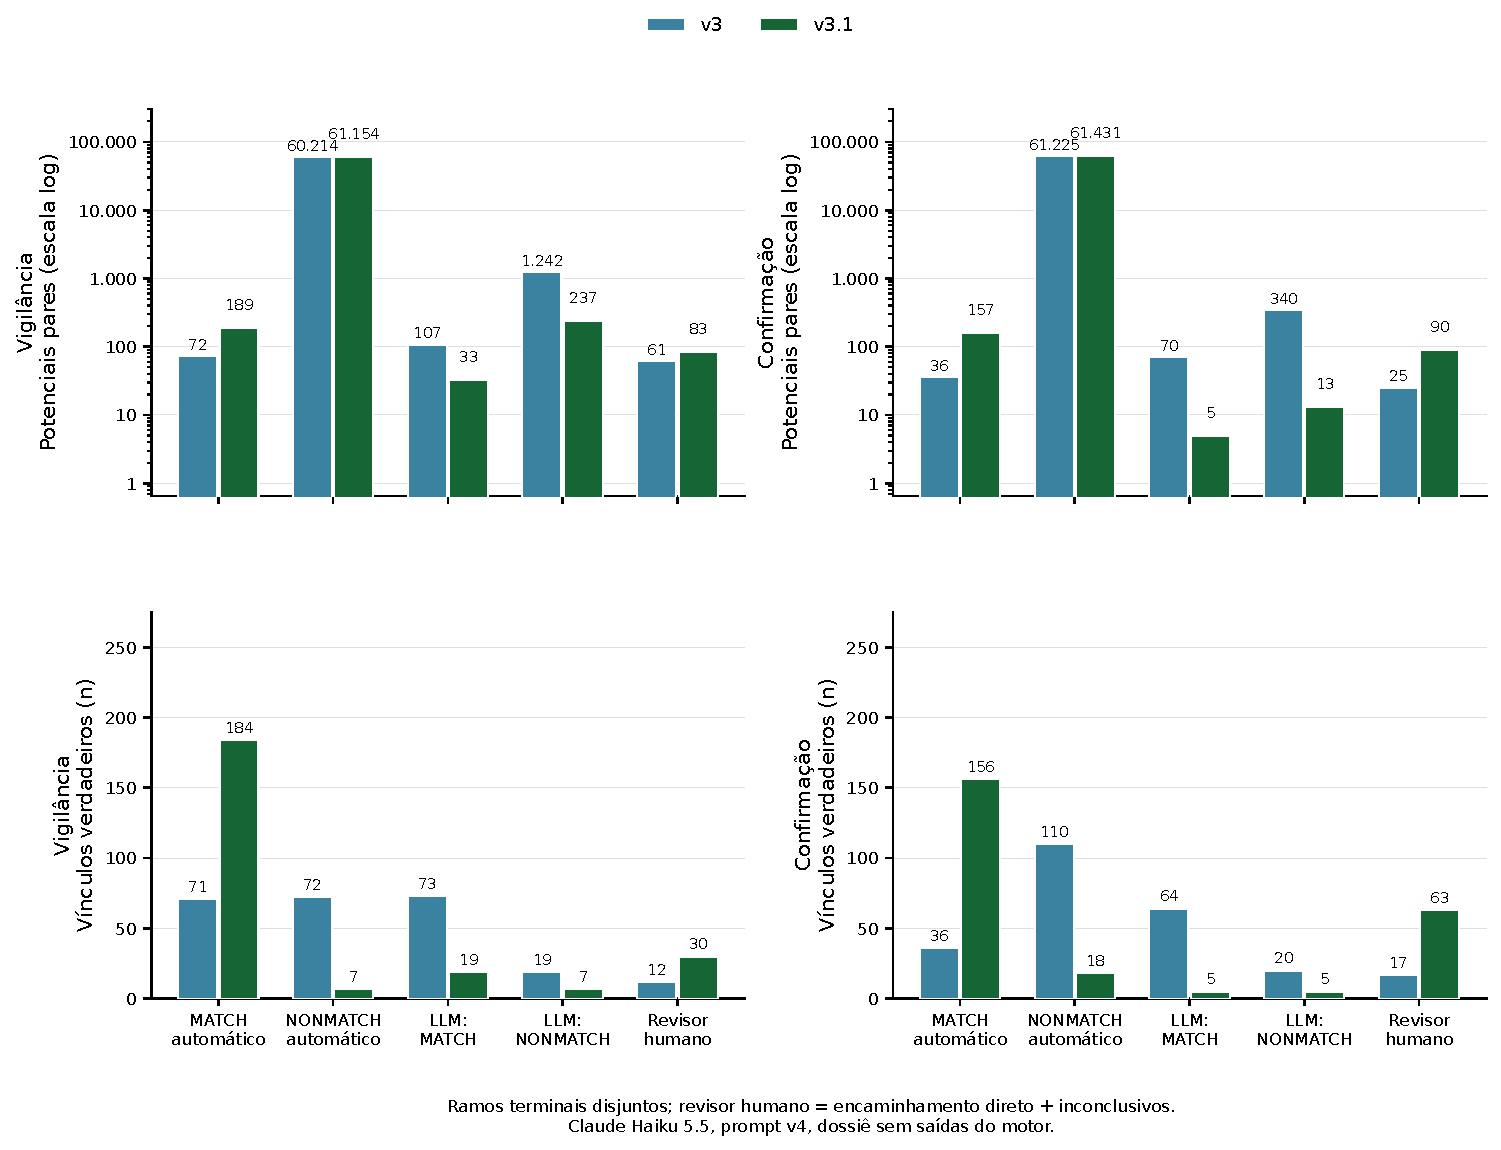
\includegraphics[width=\textwidth,height=0.75\textheight,keepaspectratio]{figures/fig_cap8_cascata_v31.pdf}
\caption{Cascata sobre a base inteira (comparação), com políticas v3 (três ações: aceitar como vínculo, rejeitar e revisão LLM) e v3.1 (quatro ações, com revisão humana distinta da revisão LLM) nos modos vigilância e confirmação e Claude Haiku 5.5 com instruções v4 (versão sem solicitação das saídas do motor) e sem as saídas do motor. LLM designa modelo de linguagem de grande porte. Os ramos apresentam contagens de potenciais pares e de pares verdadeiros segundo a referência operacional. Os ramos \texttt{MATCH} e \texttt{NONMATCH} automáticos somam as guardas (\texttt{ALWAYS}) e as decisões por custo esperado (\texttt{AUTO}); o ramo do revisor humano reúne os encaminhamentos diretos e os inconclusivos do LLM. Fonte: \texttt{data/funil\_gzcmd\_final.csv} e agregados correspondentes \cite{Jardim2026phdrepo}.}
\label{fig:cap8-cascata-v31}
\end{figure}

\section{Ablação das Medidas Contínuas de Diferença de Datas, MACD (Experimento 1)}\label{sec:e4-ap-macd}

Esta seção reúne o método e os resultados do Experimento 1, a ablação das MACD na política histórica v3.

Na ablação do GZ-CMD, foram realizadas cinco rodadas de particionamento em treinamento e teste na partição agrupada por COMPREC (registro do Sinan-TB), distinta do agrupamento por REFREC adotado na v3.1, com fração de teste de 30\% e sementes de 42 a 46, conforme as tabelas do Apêndice~\ref{sec:apendice-ablacao}. Esse protocolo difere da validação cruzada em cinco partições e do QW1 $5 \times 5$ descritos na Seção~\ref{sec:analises-complementares}. As métricas são reportadas como média e desvio-padrão entre rodadas, com comparações exploratórias por teste t pareado ($\alpha=0{,}05$). No experimento de revisão assistida, foram avaliados os 1.410 pares selecionados pelo motor v3 entre os 61.696 potenciais pares do extrato, com \textit{Platt scaling} ajustado nos próprios \textit{labels}; esse universo não representa revisão humana integral observada.

\subsection{Experimento 1: ablação e impacto das MACD}
\label{sec:e4-exp1}

A Tabela~\ref{tab:cap8-ablacao} apresenta os resultados de ablação com e sem MACD, com os valores das tabelas da Seção~\ref{sec:apendice-ablacao}, organizados por modo operacional.

\begin{table}[!ht]
\centering
\caption{Ablação restrita aos subescores e à nota final (média $\pm$ desvio-padrão, cinco divisões por COMPREC, registro do Sinan). MACD ON e OFF indicam as Medidas Contínuas de Diferença de Datas de nascimento ativadas ou desativadas. Revisões são contagens absolutas por partição de teste. As métricas são esperadas com proporções de erro do revisor fixadas na configuração v3 (política histórica de três ações: aceitar como vínculo, rejeitar e encaminhar à revisão por modelo de linguagem), não estimadas de respostas de modelo de linguagem.}
\label{tab:cap8-ablacao}
\resizebox{\textwidth}{!}{%
\begin{tabular}{|l|l|c|c|c|c|c|c|}
\hline
Modo & Configuração & VPP & Sensibilidade & F$_1$ & F$_{0{,}5}$ & F$_2$ & Revisões \\
\hline
Confirmação & MACD OFF & $0,901\pm0,033$ & $0,910\pm0,012$ & $0,905\pm0,013$ & $0,902\pm0,025$ & n.a. & $215,4\pm30,2$ \\
\hline
Confirmação & MACD ON & $0,951\pm0,004$ & $0,885\pm0,030$ & $0,916\pm0,014$ & $0,937\pm0,004$ & n.a. & $140,6\pm10,0$ \\
\hline
Vigilância & MACD OFF & $0,857\pm0,052$ & $0,936\pm0,008$ & $0,894\pm0,030$ & n.a. & $0,919\pm0,015$ & $244,2\pm43,9$ \\
\hline
Vigilância & MACD ON & $0,945\pm0,006$ & $0,938\pm0,020$ & $0,941\pm0,008$ & n.a. & $0,939\pm0,015$ & $110,0\pm7,1$ \\
\hline
\end{tabular}%
}
\par\footnotesize Fonte: \path{data/ablation_comprec_macd_allowlist_summary.csv} e \path{data/ablation_comprec_nomacd_allowlist_summary.csv}; rodadas na Seção~\ref{sec:apendice-ablacao}.
\end{table}

O experimento saneado utilizou Random Forest com 200 árvores, profundidade máxima 10 e pesos de classe balanceados, calibrado por sigmoide em validação cruzada interna de cinco partições e ajustado somente no treinamento por COMPREC, com 30\% para teste e sementes de divisão de 42 a 46. A semente do classificador permaneceu 42. Os atributos foram restritos aos 29 subescores e à nota final, acrescidos das nove MACD no braço ativado. Mantiveram-se a política v3 e as proporções de erro do revisor fixadas por faixa na configuração, não estimadas; as medidas F são esperadas, sem chamada a modelo de linguagem. O procedimento, os parâmetros e a lista de atributos estão em \path{data/ablation_comprec_allowlist_metadata.json}; as rodadas, em \path{data/ablation_comprec_macd_allowlist.csv} e \path{data/ablation_comprec_nomacd_allowlist.csv}.

Com MACD, o F$_1$ esperado foi de 0,941 na vigilância e de 0,916 na confirmação, contra 0,894 e 0,905 sem MACD. As revisões diminuíram 55,0\% e 34,7\%, respectivamente, calculadas como $100(1-\bar n_{ON}/\bar n_{OFF})$, ou 134,2 e 74,8 por partição. Nos testes t pareados, a diferença de F$_1$ apresentou $t(4)=3{,}68$, $p=0{,}021$ na vigilância e $t(4)=0{,}99$, $p=0{,}377$ na confirmação; os testes de Welch, apenas para comparação, deram $t=3{,}41$, $p=0{,}022$ e $t=1{,}32$, $p=0{,}223$. Para revisões, os valores pareados foram $p=0{,}0016$ e $p=0{,}0031$; para o VPP, $p=0{,}016$ e $p=0{,}019$; para sensibilidade, $p=0{,}776$ e $p=0{,}056$. São oito comparações exploratórias, sem ajuste de multiplicidade, produzidas por \path{scripts/exp1_testes_t.py} em \path{data/exp1_testes_t_allowlist.csv}. As cinco partições de teste se sobrepõem; o teste t pareado supõe rodadas independentes e tende a produzir valores de $p$ otimistas, que não sustentam inferência de cinco amostras independentes.

A versão anterior selecionava todas as colunas numéricas do extrato não excluídas por nome, inclusive o escore do OpenRecLink, que define PAR~=~1 pelo corte de cada passo, a situação de encerramento e identificadores. O F$_1$ esperado de 0,954 na vigilância e as reduções de revisões de 14,5\% e 17,6\%, na vigilância e na confirmação, são resultados desse caminho histórico contaminado, preservados em \path{data/ablation_comprec_macd.csv} e \path{data/ablation_comprec_nomacd.csv}, não os resultados saneados; a comparação consta de \path{data/exp1_vazamento_comparacao.csv}. A mudança não pode ser atribuída somente ao escore do OpenRecLink, porque a restrição retirou conjuntamente campos brutos, identificadores, atributos duplicados e outros derivados. A seleção saneada tampouco demonstra ausência universal de vazamento, pois a nota e os subescores permanecem relacionados à construção da referência (Apêndice~\ref{ap:sensibilidade}). Esta ablação mantém a v3; não foi refeita com a política v3.1 nem com o dossiê sem as saídas do motor. Com a mesma política v3, mas com Claude Haiku 5.5, instruções v4 e dossiê sem as saídas do motor, a cascata sobre a base inteira perdeu 91 pares verdadeiros por \texttt{NONMATCH} na vigilância, com sensibilidade automática de 58,3\% (Tabela~\ref{tab:cap8-referencia}).

\section{Registro interno do arranjo: emendas, custos e estabilidade}\label{sec:e4-ap-registro}

Esta seção documenta as emendas do registro do arranjo, os custos das execuções novas e a análise de estabilidade. O arranjo, ASR no texto, é denominado P no registro interno (\texttt{8c16a41}) e nos artefatos de \path{data/}.

No registro \texttt{8c16a41}, ASR-Platt constava entre os braços, ao lado de ASR e B1, e as sensibilidades registradas eram duas: A3, que restringe também o ajuste do classificador ao treinamento abaixo do corte, e ASR-PAR2-faixa (P-PAR2-grey no registro e nos artefatos), que estima $e_{FN}$ somente com os pares de PAR~=~2 e agrupa as quatro faixas operacionais que compõem a faixa intermediária da nota final $[5,9)$, sem usar como referência de erro os de PAR~=~1, mais fáceis. A terceira emenda, às 02:01:57 UTC de 5 de novembro de 2026, cerca de dez minutos antes da S3, autorizou as respostas do suplemento e descreveu ASR-Platt e A3 como braços de sensibilidade registrados (\path{gzcmd/prereg_arranjo_corte.yaml}, emenda 3). Essa reclassificação é desvio do registro inicial, documentado em \path{gzcmd/M_arranjo_corte_desvios.md}; o tratamento de ASR-Platt como sensibilidade que não substitui ASR decorre dela, e não do registro \texttt{8c16a41}.

A primeira emenda introduziu os alvos suavizados de \citeonline{Platt1999} e a otimização com controle de passo, porque o método de Newton saturou na primeira partição; a segunda explicitou as \textit{threads} necessárias para reproduzir as probabilidades originais fora da amostra. O suplemento autorizou respostas adicionais para ASR-Platt e A3, sem alterar braços ou custos, mas desviou da proibição inicial de chamadas de sensibilidade. A regra de parada previa mais de 500 potenciais pares pendentes em $\mathrm{ASR}\cup B1$ ou custo novo superior a US\$~2. Foram 24 potenciais pares, com US\$~0,076 estimados para a regra de parada (\path{data/arranjo_corte_s1_metadata.json}), e o consumo tarifado observado foi de US\$~0,0629, somando US\$~0,0281 na vigilância e US\$~0,0348 na confirmação. O suplemento, com 69 potenciais pares e 147 chamadas, custou US\$~0,1819 (US\$~0,1754 na vigilância e US\$~0,0066 na confirmação; \path{data/sprint3b/anthropic_sem_mo_v4_arranjo_corte_supl/execucao.json}), e o total de US\$~0,2448 soma esse valor aos US\$~0,0629 das respostas novas (campo \texttt{cost\_sources} de \path{data/arranjo_corte_metadata.json}). A regra de parada não foi acionada \cite{Jardim2026phdrepo}.

O identificador do registro inicial consta apenas no histórico do git, e a metadata \path{data/arranjo_corte_metadata.json} grava \texttt{d526c3fb}, \textit{commit} da terceira emenda, e \texttt{7b40cfb}, o da segunda.

O registro da análise de estabilidade, de 5 de novembro de 2026 às 06:19:04 UTC, é posterior à avaliação original: o critério de dominância de Pareto, com limiar de 18/20, foi fixado quando a dominância de ASR-Platt já era conhecida. O bloco de partição varia as partições e mantém fixos a semente do classificador e o número de processos paralelos; as proporções do revisor vêm das coortes congeladas, e as respostas do LLM são compartilhadas entre réplicas. A dominância de ASR-Platt exige não piorar os pares aceitos, os FP abaixo do corte, os perdidos e os encaminhamentos ao humano e ao LLM, com ao menos uma melhora. O critério de estabilidade exige pelo menos 18/20 em ambos os blocos e dominância inversa em no máximo 1/20; menos de 10/20 em ambos os blocos, ou dominância inversa em pelo menos 10,0\% em algum bloco, classifica a dominância como não sustentada.

Cada braço soma apenas o consumo registrado dos potenciais pares selecionados, com tarifas históricas, sem representar fatura do provedor. As respostas novas e as do suplemento não realimentaram as proporções congeladas do revisor.

Na faixa intermediária da nota final do CdR, que contém 151 pares verdadeiros, o corte aceita 123 e o arranjo aceitou 127 nos dois modos (84,1\%), incluindo quatro PAR~=~2, com 21 FP, 89 encaminhamentos humanos e 342 ao LLM na vigilância e quatro FP, 17 ao humano e 32 ao LLM na confirmação. A cascata sobre a base inteira aceitou 113 e 65 nessa faixa, abaixo dos 123 aceitos pelo corte, e o acréscimo automático frente ao corte isolado não elimina a perda de 13 e 27 dos 36 PAR~=~2.

O braço \textit{a posteriori} aceitou 221 e 219, com 34 e zero FP e 90 e 51 encaminhamentos humanos. A ponte B1 aceitou 194 e 131, com 40 e quatro FP. O braço A3 aceitou 219 nos dois modos, com 19 e cinco FP, e o braço ASR-PAR2-faixa aceitou 211 e 217, com 21 e zero FP.

As 242 revisões novas da análise de estabilidade tiveram custo estimado de US\$~0,6255. Somadas aos US\$~0,2448 do arranjo inicial, totalizam US\$~0,8703 (\path{data/robustez_arranjo_metadata.json}). Com os US\$~0,2633 das chamadas do filtro LLM (\path{data/filtro_llm_metadata.json}), as execuções novas somam US\$~1,13 ($0{,}2448+0{,}6255+0{,}2633=1{,}1336$), sem incluir pessoal e infraestrutura nem os cerca de US\$~76 da avaliação do Claude Sonnet 5.5 (Seção~\ref{sec:e4-ap-reavaliacao}), que não integra o arranjo.

Um checkout novo do repositório recupera o blob com finais de linha LF, não os finais de linha mistos cujo hash foi registrado, de modo que a reprodução da S1 depende do arquivo original (\path{gzcmd/S10_eol_prereg.md}). O suplemento autorizou chamadas adicionais apesar da proibição inicial de chamadas de sensibilidade, e sua declaração de ausência de mudança de parâmetros não elimina esse desvio. A reprodução numérica posterior foi descrita por concordância dentro da tolerância declarada, com partições idênticas, não por identidade de todos os bytes, e os detalhes de versões, tolerâncias, testes e execução estão em \path{gzcmd/M_arranjo_corte_desvios.md}.

Na análise de estabilidade, a validação da identidade dos dossiês ficou restrita à rotina adicional de execução, e a leitura das respostas congeladas não verificava integralmente seu vocabulário e completude. Essas limitações de controle estão documentadas em \path{gzcmd/M_robustez_arranjo_desvios.md}.

\section{Complementos posteriores ao registro do arranjo}\label{sec:e4-ap-posteriores}

Esta seção reúne complementos posteriores ao registro do arranjo: a definição dos atributos de contexto, o contraste entre os resultados históricos e os de Claude Haiku 5.5 com instruções v4, o escopo do dossiê e os limites do consenso entre agentes.

Os atributos de contexto por óbito e por registro candidato (Seção~\ref{sec:e4-mesma-carga}) são o número de candidatos, a posição pela nota final, as diferenças para a melhor e a segunda nota e o indicador de melhor candidato.

Os resultados históricos da revisão assistida por LLM (Seção~\ref{sec:e4-llm-inicial}) não equivalem aos resultados com Claude Haiku 5.5, instruções v4 e dossiê sem as saídas do motor. No arranjo, os lotes foram de 344 e 41 potenciais pares, com sensibilidades automáticas da cadeia de 87,0\% e 88,7\% e perdas de 13 e 27 pares verdadeiros. Na cascata sobre a base inteira, foram 347 e 44, com sensibilidades de 78,5\% e 53,4\%. A diferença de aceitação total decorre dos 211 PAR~=~1 preservados pelo arranjo por construção, não de melhor recuperação abaixo do corte, e esses valores descrevem decisões da cadeia, não o desempenho isolado do modelo \cite{Jardim2026phdrepo}.

O dossiê histórico contém subescores numéricos de similaridade, probabilidades e indicadores derivados, sem os campos textuais originais, e a retirada das saídas decisórias do motor distingue o dossiê final e decorre da investigação de ancoragem, não da inclusão de dados identificáveis. Arquiteturas de \textit{entity matching} como DeepMatcher e DITTO utilizam representações textuais, mas não foram avaliadas como alternativas nessa cascata \cite{Mudgal2018deepmatcher,Li2020ditto,Jardim2026phdrepo}.

O consenso entre agentes não estabelece independência do motor nem repetibilidade: Claude Haiku 5.5 é estocástico, e as mudanças de dossiê e instruções impedem atribuir diferenças apenas ao modelo. O custo estimado foi de US\$~0,94 e US\$~0,11 no arranjo, contra US\$~0,92 e US\$~0,12 na cascata sobre a base inteira, sem pessoal ou infraestrutura, e os encaminhamentos humanos da comparação, 111 e 127, constituem trabalho pendente, não acertos observados \cite{Jardim2026phdrepo}.

\section{Dossiê ampliado v5 e réplicas entre modelos}\label{sec:e4-ap-dossie}

Esta seção complementa a comparação de modelos de tamanhos distintos e o exame com o dossiê ampliado v5, descritos no corpo do capítulo (Seção~\ref{sec:e4-tamanho-modelo}), em que os estratos V1 e V2 estão definidos. Os modelos são Claude Haiku 5.5, Claude Opus 5.5 e Claude Fable 5.1, designados a seguir por Haiku, Opus e Fable.

As diferenças entre modelos coexistem com variação entre réplicas: na vigilância, o Haiku passou de 21 para 19 aceitações em V1 nos 21 casos completos da réplica, enquanto Opus e Fable variaram de 21 para 20 e de 22 para 21 nos 25 pares, amplitude comparável às diferenças entre modelos, sem teste formal dessa equivalência. Em V2 (pares verdadeiros PAR~=~2 não aceitos pelo Haiku), Opus e Fable produziram, respectivamente, oito e nove descartes, contra seis do Haiku, observação descritiva de maior cautela nos PAR~=~2 difíceis, sem aumento uniforme dos inconclusivos (\path{data/probe_frontier_agregado.csv}). Os custos por par da Tabela~\ref{tab:cap8-tamanho-modelo} distinguem os transportes e as execuções históricas e não isolam o efeito do tamanho sobre a despesa.

No exame com o dossiê ampliado, os três FP que deixaram de ser \texttt{MATCH} passaram todos a \texttt{UNSURE}, o VPP da confirmação permaneceu igual ao da v4 e a perda de resposta atingiu seis dos 13 pares verdadeiros de V2. O lote de vigilância foi cancelado por prazo do crédito, mas suas 299 respostas tardias bem-sucedidas foram utilizadas e não repetidas, e o custo por consumo, incluindo piloto e respostas truncadas, foi de US\$~0,32. Claude Opus 5.5 não foi executado, conforme a regra de acionamento. As comparações entre modelos usaram raciocínio adaptativo padrão da API, que não pôde ser desligado no Opus 5.5 nem no Fable 5.1 (\path{data/probe_dossie_v5_metadata.json}).
